\documentclass[a4paper]{book}
\usepackage{imakeidx}
\usepackage{graphicx}
\usepackage{amsmath}
\usepackage{amsthm}
\usepackage{amsfonts}
\usepackage{amssymb}
\usepackage{booktabs}
\usepackage[T1]{fontenc}
\usepackage[utf8]{inputenc}
\usepackage[english]{babel}
\usepackage[hidelinks]{hyperref}
\usepackage{mwe}
\usepackage{float}
\usepackage{subfig}
\usepackage{array}
\usepackage{soul}
\usepackage{multirow}
\usepackage{tikz}
\usetikzlibrary{arrows,automata}
\newcommand{\tableline}[1]{
  \begin{tabular}{@{}c@{}}\strut#1\strut\end{tabular}
}
\newcommand*\circled[1]{\tikz[baseline=(char.base)]{
            \node[shape=circle,draw,inner sep=2pt] (char) {#1};}}
\makeindex[columns=2, title = Alphabetical Index, options= -s style.ist]

\newtheorem{theorem}{Theorem}[chapter]
\newtheorem{corollary}{Corollary}[theorem]
\newtheorem{definition}{Definition}[chapter]
\newtheorem{property}{Property}[chapter]
\newtheorem{algorithm}{Algorithm}[chapter]

\begin{document}
	\author{Luca Alessandrini, Elia Ravella, Juri Sacchetta}
	\title{FLC defucked version}
	\maketitle
	\tableofcontents
	\chapter{Regular Expressions and Regular Languages}
    \section{Introduction}
        Regual languages are the simplest family of formal language.
    \section{RL and RE}
        \subsection{Introduction and Definitions}
            A Regular Language is a \textbf{language over an alphabet that can be expressed by applying} \emph{a finite number of times} this three operations:
            \begin{enumerate}
                \item Union $\bigcup, \vee$
                \item Concatenation $\cdot$
                \item Star (Kleene Star)
            \end{enumerate}
            Rule of precedence: star, concatenation, union.
            It is permitted to use $\varepsilon = \emptyset^* $
            
            \begin{definition}[Regular Language]
                A language is regular  if it is the meaning (hence if it is generated) by a regular expression.
            \end{definition}
            \begin{definition}[Family of Regular Languages (REG)]
                Collection of regular languages.
            \end{definition}
            \begin{definition}[Family of Finite Languages (FIN)]
                Collection of all languages of finite cardinality.
            \end{definition}
            \textbf{Caution}: REG and FIN are sets of sets of set of strings, not set of strings themeselves.

            Notice that \emph{every finite language is regular} because it is the (finite)
            union of finitely many strings, and each string is in turn the concatenation
            of finitely many letters or in general of alphabetic symbols

            \begin{equation*}
                \left(x_1\bigcup x_2\bigcup\ldots\bigcup x_k\right)=\left({a_1}_1{a_1}_2\ldots {a_1}_n\bigcup\ldots\bigcup{a_k}_1{a_k}_2\ldots{a_k}_n\right)
            \end{equation*}

            Remember that $FIN\subset REG$
        \subsection{Subexpression of a regexp}
            \begin{enumerate}
                \item Consider a fully parenthesized regex
                \begin{equation}
                    e=\left(a\bigcup\left(bb\right)\right)^*\left(c^+\bigcup\left(a\bigcup\left(bb\right)\right)\right)
                \end{equation}
                \item Number every alphabetic symbol that occurs in the regexp
                \begin{equation}
                    e_N=\left(a_1\bigcup\left(b_2b_3\right)\right)^*\left(c_4^+\bigcup\left(a_5\bigcup\left(b_6b_7\right)\right)\right)
                \end{equation}
                \item isolate the subexpressions and put them into evidence
            \end{enumerate}



        \subsection{Other Operators}
            Also set operators can be used: Intersection and Complement are used when it's more concise to express a language to a set of languages (the former) or 
            the inverse of a complex rule (the latter: a clear example is "a language with no 2 consecutive 'a' in it").
        
        To define a Regular Language formally a \emph{Regular Expression} is used, defined as a string of either elements of the alphabet or operators that symbolize 
        the three operation for regular languages.
        The Derivation Relation binds the RE with its productions: in fact, an expression is said to be \emph{derived} from another one if it's totally or partly a 
        choice of another one. A choice is an alternative between two options that the RE gives you (a union operator poses a choice). A Language is defined as the 
        set of all possible productions that can be derived from a RE.

    \section{Ambiguity}
        \subsection{General Concept}
        Easy enough: a RE is ambiguous if more than one identical productions exists. This obviously leads to problems in the parsing procedure, due to the difficulty 
        to "trace back" the choices that has been made to get to that point. 
        \begin{definition}[Ambiguity Degree of a String]
            Referring to a single string belonging to a language, is the number of different possible sintax trees generating that same string.
        \end{definition}
        \begin{definition}[Ambiguity Degree of a Grammar]
            It is the maximum degree of ambiguity of the strings obtainable from the grammar.
        \end{definition}
        \subsection{Formal proof}\label{sect:formalproofambiguity}
            TODO%//TODO: controlla dove mettere questa sezione, e prima vanno capiti i parser

    \section{Closure Property}
        Pretty straightforward, is the same "closure" concept from classic algebra; a family of languages is closed under an operator if applying n times that 
        operator to a language of that family obtains only languages of that family. You can't "exit that family" with that operator.
        
        The REG(ular) family of languages is closed under
        \begin{itemize}
            \item concatenation
            \item union
            \item star
        \end{itemize}
        Therefore is closed also under derived operators from these (cross).

	\chapter{Context Free Grammars}
	\section{Preliminar definitions}
		Regular expressions as a tool to generate languages are not enough powerful. 
		Super simple languages like "all words followed by their reverse" or "concatenation of two strings of the same length" cannot be generated.

		Context Free grammars are defined by means of four entities
		\begin{itemize}
			\item $V$: \emph{non-terminal alphabet}, is a set of \emph{non-terminal symbols (or syntactic classes)}
			\item $\sum$: \emph{terminal alphabet}, is the set of the \emph{characteres} that costitute the phrases
			\item $P$: is a set of \emph{syntactic rules} (also called \emph{production rules} or simply \emph{rules})
			\item $S \in V$ is a particular non-terminal, called axiom
		\end{itemize}
		One particular nonterminal is choosen as starter (or axiom).
		A Rule is an ordered pair with a left side and a right side: left side can contain only nonterminals, right side both terminals and nonterminals. 
		
		In order to define a language, one can use RULES that, after repeated application, allow to generate all and only the phrases of the language
		The set of such rules constitutes a GENERATIVE GRAMMAR (or SYNTAX).

		\begin{definition}[Regular Language]
			A set of rules generating all the possible strings belong to the language.
		\end{definition}


		\subsection{Rule Classification}
			Lowercase or greek letters: terminals.\\
			Uppercase letters: terminals.
			\begin{definition}[Recursive]
				A $\rightarrow$ $\alpha$ A $\beta$ 
			\end{definition}
			\begin{definition}[Left recursive]
				A $\rightarrow$ A $\beta$ 
			\end{definition}
			\begin{definition}[Right recursive]
				A $\rightarrow$ $\alpha$ A
			\end{definition}
			\begin{definition}[Copy]
				A $\rightarrow$ B
			\end{definition}
			\begin{definition}[Linear]
				At most one nonterminal on the right side.
			\end{definition}
			\begin{definition}[Right Linear]
				Linear + nonterminal is suffix.
			\end{definition}
			\begin{definition}[Left Linear]
				Linear + nonterminal is prefix.
			\end{definition}
			\begin{definition}[Chomsky]
				Right side is either two nonterminals or a terminal.
			\end{definition}
			\begin{definition}[Greibach normal]
				Right side starts with a terminal symbol.
			\end{definition}
			\begin{definition}[Operator normal]
				A $\rightarrow$ B c D.
			\end{definition}
    \section{Grammar Cleaning}
        Writing a grammar following non-grammar rules (so doing it for a purpose and not for its own sake) can lead to useless rules or unreachable 
		terminals or nonterminals. This is prevented by the Grammar Cleaning algorithm:
            \begin{enumerate}
                \item Compute the well-defined nonterminals (the ones that are "reachable from the production")
                \item From the well defined nonterminals build the production tree (such a rare technique in computer science) and check if there are nonterminals in 
				the nonterminal alphabet that are not reachable from the axiom.
                \item (Optional but useful) Check for circular derivation like A $\rightarrow$ A $\rightarrow$ x
            \end{enumerate}
    
    \section{Infinite Grammars}
        A grammar is said to be infinite\\
        $\Leftrightarrow$\\
        A grammar has a recursive production\\\\
        The grammar is assumed to be clean and free from circular derivation. 
       
    \section{Syntax Trees}
    	The production procedure can be visualized by a tree (how strange) where every arch represents a symbol of the right part (or a choice for it). They're 
		regular trees (so connected directed acyclic graphs) but the nodes on the same level (or at least sons of the same father) are ordered from left to right.

    	The degree or arity of a node is the number of its \emph{siblings} (and not of his sons, that's more intuitive). The \emph{frontier} of the tree is the 
		sequence of all leaves. \underline{A syntax tree has the axiom as the root and a sentence as the frontier}.

    	\textbf{Remember:} a syntax tree represents \textbf{a single production} and not all possible ones.
	
	\section{Ambiguity}\label{sec:ambig}
		Ambiguity\index{Ambiguity} in grammars is similar to the ambiguity for regular expressions. The definition is pretty much the same: a sentence is ambiguous 
		if it admits several different syntax trees.

		Syntactic ambiguity (the only of interest when studying formal languages) is the kind of ambiguity that derives from the \emph{structure} of the production, 
		rather than the effective meaning it carry.% //TODO metti in risalto sta cosa

		The formal problem of discovering/computing the ambiguity of a grammar is an undecidable one. This is in practice not a great problem: heuristics to check 
		if a given grammar is ambiguous exists, but most importantly the grammar designer should keep in mind (and design accordingly) the said grammar in an 
		unambiguous way.
		
		\subsection{Ambiguous Forms and Remedies}
		% //TODO metti una description o fai capire che stai per elencare i tipi 
			\subsubsection{Bilateral Recursion}
				A bilateral recursion (so a both left and right recursive rule) often leads to ambiguity because there's usually no fixed order of generation 
				of nonterminals.

				This can be usually avoided by splitting the two side recursive rule into more rules each one either right or left recursive.

			\subsubsection{Ambiguity from Union}
				Pretty straightforward: if two different languages can generate the same sentence, the union of these languages is ambiguous by construction.

				To cope with such problem, often a full redesign of the grammars is needed.
			\subsubsection{Ambiguity from Concatenation}
				Concatenating two (or more) languages can be a problem if a suffix of a language is a prefix in a language that follows it.

				To remove this kind of ambiguity, it's sufficent to add an extra separator character between languages.
			\subsubsection{Ambiguity in Conditional Phrase}
				The infamous "dangling else problem" is an ambiguity problem that falls in this category. Generally this kind of ambiguity arises when more 
				variants are accepted for the same language structure, and no particular delimiter for parts is provided.

				Usually removed by adding delimiters (endif, fi)
			\subsubsection{Inherent Ambiguity}
				An inherent ambiguous language is generated by a set of grammar in which \emph{all} the grammars are ambiguous
	
	\section{Closure Property}
		The CF languages (so all languages generated by Context Free grammars) are closed under the operations of
		\begin{itemize}
			\item union
			\item concatenation
			\item star
		\end{itemize}
		
		\subsubsection{Complement and Intersection}
			Let L and L2 be regular languages. Their intersection and the complement of each is still a regular language. (The formal proof utilizes the 
			recognizers automata to prove this).
	
	\section{Equivalence}
	%//TODO metti una fottuta spiegazione su che cose un condensed tree
		Two grammar are said to be equivalent if they define the same language. Two grammars are \emph{strongly} equivalent if they define the same language 
		\textbf{and} they have the same \emph{condensed} \emph{skeleton} \emph{trees}; this means that every production from both grammar is generated 
		"with the same choices".

		Strong equivalence $\Rightarrow$ weak equivalence

		Strong equivalence can be formally proved, while checking for weak equivalence is an undecidable problem.

		\subsubsection{Structural Adequacy}
			The difference between strong and weak equivalence is not only a formal one: if we consider (for example) the generation of arithmetic expression 
			(that should take into account also the operator precedences) only the grammar with the syntax tree that respects the precedences, and all the 
			\emph{strongly equivalent} ones, will be structurally adequate.

				\begin{figure}
					\centering
					\begin{minipage}{0.45\textwidth}
						\centering
						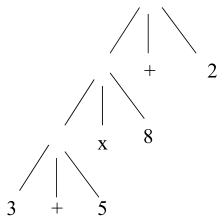
\includegraphics[width=0.9\textwidth]{./images/structAdeq1.png}
				    	\caption{Structurally inadequate syntax tree: it can be seen how the operator precedence is not respected}
					\end{minipage}\hfill
					\begin{minipage}{0.45\textwidth}
						\centering
						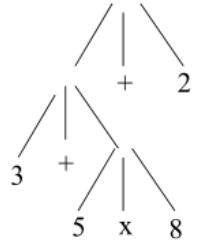
\includegraphics[width=0.9\textwidth]{./images/structAdeq2.png} 
				    	\caption{Structurally adequate tree}
					\end{minipage}
				\end{figure}
			
	\section{Grammar Transformation and Normal Forms}
	%//TODO controllare se c'è tutto, sembra un po' sintetico
		Normal forms are standardized rules. They don't reduce grammar expressiveness of the grammar, and using them does not affect the language iself. They just 
		guide the design process to obtain a grammar with certain properties.

		\subsubsection{Elimination of the axiom from right part}
			Straightforward. Use an additional rule from the axiom to a sub-axiom that is replaced in all other rules.
		\subsubsection{Nullable nonterminals and empty rules}
			A nonterminal is nullable if exists a derivation from said nonterminal to the empty string. To eliminate them, eliminate all the empty productions 
			from the right part of the rules, substituting them with the non-empty sub productions.
		\subsubsection{Copy rules}
			Copy rules are rules in the A $\rightarrow$ B form, with both A and B nonterminals. An algorithm to eliminate copy rules functions this way:
			\begin{enumerate}
				\item A set \emph{Copy(A)} is defined, that contains all the transitive copies of A and A itself
				\item \emph{Copy(A)} is filled with all the nonterminals that are copies (direct or indirect) of A, so that a straight derivation A $\rightarrow$ C 
				exists
				\item The ne set of rules is defined, eliminating all the productions from A to the nonterminals that are in \emph{Copy(A)}.  
			\end{enumerate}
			The above algorithm should take into consideration that a production A $\rightarrow$ BC can be a copy production if either B or C are nullable. Often 
			it's assumed a nonnullable grammar.
		\subsubsection{Recursion conversion}
			Another important class of grammars is the nonleft-recursive. Right recursive grammars are preferred because their laguage is simpler to parse. To 
			transform a left recursive rule to a right ecursive an algorithm has been designed:
			\begin{enumerate}
				\item Identify all the recursive rules of form A $\rightarrow$ A $\gamma$
				\item Add an auxiliary nonterminal X and add the set of rules X $\rightarrow$ $\gamma$ X; the expansion of A becomes A $\rightarrow$ $\alpha$ X, 
				where $\alpha$ is a possible production obtained from A.
			\end{enumerate}
			Now all the immediate l-recursive rules are taken care of.
		\subsubsection{Chomsky normal form}
			Only two possible types of rules: homogeneous binary (nonterminal to two nonterminals) or terminal with singleton right part (nonterminal to single 
			terminal). If the empty string is in the language, it can only appear as an axiomatic production, and the axiom cannot appear in \emph{any} right part.

			Obtaining a Chomsky grammar:
			\begin{enumerate}
				\item all non binary rules are converted to binary: the first non terminal is singled out 
				\item and all the others are replaced by another additional nonterminal, which is added to the nonterminals alphabet and has as production only 
				the one that generates all the leftover nonterminals from passage 1
				\item passages 1 and 2 ainherently recursive
				\item to cope with the rules that have both terminal and non terminals in the right part, the terminals are simple replaced with singleton 
				nonterminals
			\end{enumerate}
		\subsubsection{Greibach and real-time forms}
			Real time grammars are grammars where each right part begins with a terminal symbol. If the additional costraint "the right part could contain exactly 
			one terminal followed by zero or more nonterminals" we obtain a Greibach normal grammar.
			 
	\section{Extended Context Free Grammars}
		They're simply context free grammars (also called Backus Normal Form -> BNF) extended with the regular expression's operation such as star, and union 
		operation. The closure of the CF family under this two operations renders this exension as a merely aesthetic improvement, because the expressiveness 
		remain unchanged.

		The language of a ECF grammar is generated as the one of a CF grammar; the only effect the regular expansion has on the syntactic trees is an augmentation 
		of the breadth and a decrease in the height. This is a further improvement to readability.
	
	\section{Grammar of regular languages}
		As previously stated, regular languages (generated by regular expressions) are a proper subset of context free languages (generated by a context free 
		grammar). This means that there's a one-to-one correlation between regular expression and a grammar that expresses the same language. 
		\subsection{Unilinear Grammars}
		\label{sec:uni_linear_grammars}
			A grammar is said to be linear if every rule of that grammar is in the A $\rightarrow$ uBv form, where A and B non terminals (B can also be $\epsilon$) 
			and u and v terminal symbols.

			If only one of the two terminals is present the grammar is said to be right- or left-linear, wheter the nonterminal is right or left side of the 
			terminal symbol.

			A grammar where all rules are either right or left linear is said unilinear. A strict unilinear grammar has only one terminal per side of the rule.
			\begin{property}[Relation with regular expressions]
				Regular languages are a subset of unilinear languages: REG $\supseteq$ UNI; moreover, from an uniliear grammar we can always derive a regular 
				expression with the same expressiveness $\Rightarrow$ UNI $\supseteq$ REG. We obtain (IMPORTANT) UNI $\equiv$ REG.
			\end{property}
		\subsection{Linear Language equations}\label{sect:linlangeq}
			We want to go from a set of gramamr rules to the complete language generated. To do this we analyse the problem as a problem of languages where the 
			admitted operation is the union of sub-languages.
			Let $n = \lvert V \rvert$ be the number of nonterminals of grammar $G$. Each nonterminal $A_i$ is defined by a set of alternatives:

			$$Ai \longrightarrow a A_1 \vert b A_1 \vert \cdots \vert a A_n \vert b A_n \vert \cdots \vert A_1 \vert \cdots \vert A_n \vert \varepsilon$$
			some of which may also be missing. We write the corresponding linear equation:
			$$L_{A_i} = a L_{A_1} \bigcup b L_{A_1} \bigcup \cdots \bigcup a L_{A_n} \bigcup b L_{A_n} \bigcup \cdots\bigcup L_{A_1} \bigcup \cdots \bigcup 
			L_{A_n} \bigcup \varepsilon$$
			The last term disappears if the rule does not contain the alternative $A_i \rightarrow\varepsilon$.
			
			Practical example: \ref{ese:linlangeq}.
	\chapter{Finite Automaton as Regular Language Recognizers}
	\section{Preliminar definitions}
	You should know what a FSA is. In particular, you should know well DFSAs

	A Finite State Machine (or finite state automaton) is composed of a set of states, a transiction function (that determines the change of state at a certain input) a 
	set of termination states, and an input alphabet.

	\textbf{\underline{A DFSA is expressive as an unilinear grammar}} (so like a regular expression).

	What we want to do is to use FSA as parsers to determine if a specific string belongs to a language.
	\begin{definition}[Accepted / Regognized string]
		a string x is accepted (recognized) iff the automaton,
		starting from initial configuration with x $\dashv$ as input
		performs a computation and reaches a final configuration
	\end{definition}

	From FSA theory we can state that a computation ends when the automaton:
	\begin{itemize}
		\item raches a final configuration ($\Rightarrow$ string is accepted), or
		\item no move can be executed ($\Rightarrow$ string not accepted)
	\end{itemize}

	\begin{definition}[Equivalent automata]
		Two automata accepting the same language are called equivalent.
	\end{definition}

	\begin{definition}[String recognized]\label{def:recstr}
		A string $x$ is recognized (or accepted) by automaton $M$ if and only if when scanning $x$, $M$ goes from the initial to the final state.
	\end{definition}

	\begin{definition}[Language recognized]
		A Language is recognized by automaton $M$ if all its strings are recognized\footnote{See definition \ref{def:recstr}.}
	\end{definition}

	\begin{definition}[Finite-state recognizable]
		The family of languages accepted by finite state automata is called finite-state recognizable.
	\end{definition}

	\begin{definition}[Completed FSA]
		The transition function can always be made complete by means of an \textbf{error state} $q_{err}$:
		\begin{align*}
			\forall \mbox{ state } q\in Q \mbox{ and } \forall \mbox{ symbol } a\in\Sigma\\
			\mbox{ if } \delta\left(q,a\right) \mbox{ is undefined }\\
			\mbox{ and } \forall \mbox{ symbol } a\in \Sigma \mbox{ let } \delta \left(q_{err},a\right)=q_{err}
		\end{align*}
	\end{definition}
	\section{Clean automaton}\label{sect:cleanautom}
		A state can be useful or useless. A state is useful if it is reachable from an initiale state and a final state can be reached from it (condition of 
		accessibility and post-accessibility). Otherwise it's useless.
		\begin{property}
			For every finite automaton there exists an equivalent clean automaton.
		\end{property}
		To clean an automaton it can be easily flooded starting from the initial state then starting from the final state(s); all states not flooded at the end are 
		useless.
	
		\begin{definition}[Undistinguishable states]\label{def:undiststates}
			Two state are undistinguishable if applying the same input to the both reach a final state or both do not.
		\end{definition}
		 This relation looks like it does not provide a tool to effectively 
		distinguish two state, but it's a RECURSIVE DEFINITION:
		\begin{itemize}
			\item The sink state (or error state) is distinguishable from all other state;
			\item If a state is final is distinguishable from every other non final state;
			\item Two states are distinguishable \textbf{if their next state is distinguishable}.
		\end{itemize}
		\textbf{Note}: State $p$ and state $q$ are different (and distinguishable) if the set of labels of the arcs outgoing from $p$ and $q$ are different.

		\emph{Indistinguishability} is a binary \textbf{relation}; it is \textbf{reflexive}, \textbf{symmetric}, and \textbf{transitive} hence it is an 
		\textbf{equivalence relation}.

		\subsection{Minimization}
			States of the minimal automaton $M'$: the \emph{equivalence classes of the indistinguishability relation} transition function, arcs among equivalence 
			classes:
			$$[\ldots,p_r, \ldots] \overset{b}{\longrightarrow} [\ldots, q_s, \ldots] \Rightarrow [p_r] \overset{b}{\longrightarrow} [q_s]$$
			\begin{property}[Minimal automaton - uniqueness property]
				For every finite state language, the finite recognizer is minimal w.r.t. the number of states exists and is unique (apart from a renaming of states)
			\end{property}
			This property enables to represent a whole class of equivalent automata with a single one, that moreover is \emph{minimal}.

			An algorithm to reduce automaton to their minimal equivalent is based on the equivalence relation between states called \emph{distinguishablity}.	
	\section{Nondeterministic Automata}
		As a unilinear grammar rule can contain multiple alternatives for the same nonterminal, a FSA can have multiple states associated to a input symbol.
		Moreover, an automaton could also have spontaneous moves, so arcs that are not associated with any kind of input, besides the empty string.
		
		%//TODO re-write definition of NFSA
		If one or both these two kinds of situation happen to be in a FSA it's called nondeterministic, due to the nondeterminism of the output (same input can lead 
		to different output).

		There are a few motivations to add nondeterminism to an automaton:
		\begin{itemize}
			\item Concision: a nondeterministic automaton is often smaller than his deterministic counterpart, rendering the former more readable
			\item Mapping to grammars: as said, multiple alternative rules are more easily mapped on a NFSA than on a FSA
			\item Language reversing: when reversing an automaton (so changing arrows direction and initial/final states) nondeterminism often pops out
			\item ND recognizers: NFSA can be used to draft out a recognizer automaton
		\end{itemize}
		\subsection{Elimination of nondeterminism}
			The final implementation of a recognizer automaton must be deterministic (for now).
			\begin{theorem}\label{th:NFSA_TO_DFSA}
				Every nondeterministic automaton can be transformed in a deterministic equivalent one.
			\end{theorem}
			The theorem~\ref{th:NFSA_TO_DFSA} lets to the definition of:
			\begin{corollary}
				Every unilinear grammar\footnote{See section: \ref{sec:uni_linear_grammars}}  admits a equivalent nonambiguous one.
			\end{corollary}
			We focus on removing spontaneous moves to do we introduce:
			\paragraph{Backward propagation method}
				\begin{enumerate}
					\item Compute the transitive closure of $\epsilon$ moves: if three states are connected sequentially by spontaneous moves, add all the $\epsilon$ 
					moves that shows all the $\epsilon$ paths.
					\item Backward propagation of the scanning moves over the epsilon moves: if a path contains a normal scan move AND a spontaneous move, then 
					connect the first and last states of that path with a scan move with the element scanned.
					\item Add all the states that spontaneously arrive to the final state to the final states set.
					\item Delete all $\epsilon$ moves left.
				\end{enumerate}
				
			\begin{definition}[Ambiguity]
				As for the grammars, an automaton is ambiguous if it accepts a string with two different computations. 
			\end{definition}
	
	\section{Automaton to regexp - Brzozowski McCluskey method}
		The Brzozowski McCluskey method (BMC) method allows to generate a regular expression from an automaton that produces the same language.\\
		Assumptions:
		\begin{itemize}
			\item unique initial state
			\item initial state has no incoming arcs
			\item unique final state
			\item final state has no outgoing arcs
		\end{itemize}
		%The algorithm is quite simple: at every step, an internal node is removed and substitued by a set of arcs labeled as regular expressions (the additional 
		%arcs must not modify the automaton behaviour, obiously. They should compensate with the regexp the introduce the lack of the removed state). 
		%The algorithm terminates when only initial state and final state are left, so one only arc with a single regexp, equivalent to the whole automaton.
		Before seeing the algorithm, we need to consider the initial state $i$, the final state $t$ and define internal states.
		\begin{definition}[Internal states]
			Every state other than initial state $i$ and final state $t$ is called \textbf{internal}.
		\end{definition}
		\begin{algorithm}[Brzozowski McCluskey (BMC) method]
			\begin{itemize}
				\item[]
				\item If initial state $i$ has arcs incoming, add a new initial state with a spontaneous move ($\varepsilon$ move) to the original initial state. Do 
				the similar thing to the final state $t$ if it has others outgoing arcs (note that now the ex-initial node and the ex-final node have become 
				\emph{internal}).
				\item Until there are internal nodes:
				\begin{itemize}
					\item Consider an internal node to be removed;
					\item Construct an equivalent automaton (called \emph{generalized}), which will be more flexible because it allows the arc labels to be not just
					terminal characters, but also regular languages (labels can be r.e.).
				\end{itemize}
			\end{itemize}
			Once every node has been eliminated, we are left with only two nodes ($i$,$t$) and one arc. At this point, the label of the arc $i\longrightarrow t$ is the 
			r.e. of the language.
		\end{algorithm}
		Notes for nerdier people: this methods is similar (if not the same) to the one used to pass from an unilinear grammar to a regexp making use of "linear 
		language equations".
		\begin{figure}[htp]
			\centering
			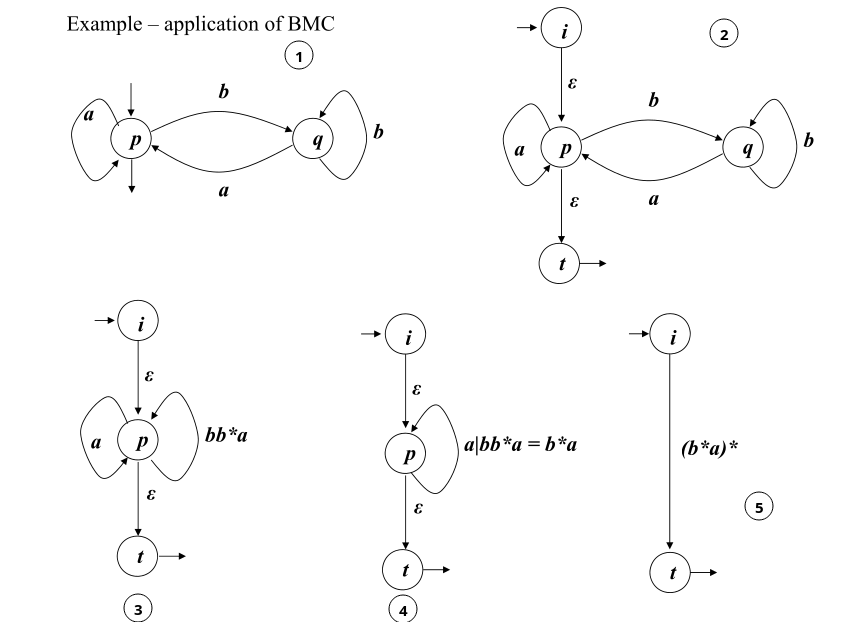
\includegraphics[width = \textwidth]{./images/BMCMethod.png}
		\end{figure}
	
	\section{Regexp to non deterministic recognizer - the Thompson Structural Method}
		Thompson's method analyzes a regexp by simple parts and generates the components associated to them. It then interconnects the components to build the whole 
		automaton. A parallel is drawn between the operators in a regexp and the finite state components they generate.
		\begin{itemize}
			\item An \textbf{atomic expression} is just translated as an arc between two states. The empty string is considered an atomic expression.
			\item \textbf{Concatenation} is expressed as a spontaneous move that connects two states, a single epsilon arc.
			\item On the other hand, \textbf{alternatives} are parallel blocks of states; all blocks connected to a single entry state and a single exit state 
			through epsilon moves.
			\empty The \textbf{star closure} instead is built as a recursive block of components, encapsulated in a initial and final state. The extreme steates 
			are connected by a epsilon move.
		\end{itemize}
		Example:
		\begin{figure}[H]
			\begin{center}
			    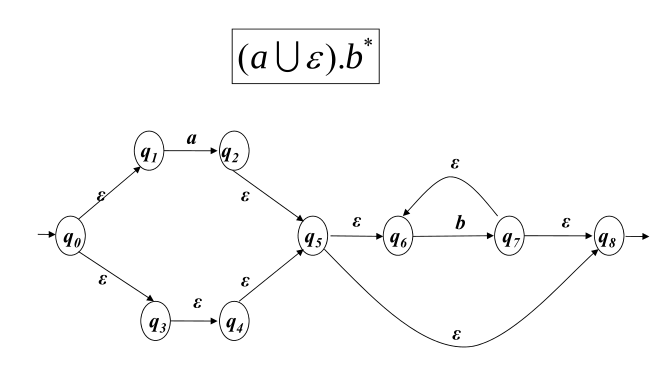
\includegraphics[width = \textwidth]{./images/ThompsonMethod.png}
			\end{center}
		\end{figure}
		
	\section{Regexp to deterministic automaton - Berry Sethi Method}
		\subsection{Theorical fundament: local languages and local automata}
		%//TODO check the theory of local languages -> still missing how to recognize if s.thing is local and local automaton (definitions useful for practical 
		%exercises)
			In order to fully understand the Berry Sethi method (ahaha) we must introduce the family of local languages.
			\begin{definition}[Local sets]
				For a language $L$ over an alphabet $\Sigma$, the set of \textbf{initials} is:
				$$Ini(L)=\lbrace a\in\Sigma\vert a\Sigma^*\cap L\neq\emptyset\rbrace$$
				i.e., the starting characters of the sentences. The set of \textbf{finals} is:
				$$Fin(L)=\lbrace a\in\Sigma\vert \Sigma^* a\cap L\neq\emptyset\rbrace$$
				i.e., the ending characters of the sentences. The set of \textbf{digrams} (factors) is:
				$$Dig(L)=\lbrace x\in\Sigma^2\vert\Sigma^*\times\Sigma^*\cap L\neq\emptyset\rbrace$$
				i.e., the substrings of length two present in the sentences. The three sets abve are called \textbf{local}.
				The complementary of digrams are:
				$$\overline{Dig(L)}=\Sigma^2/Dig(L)$$
			\end{definition}

			\begin{definition}[Local language]
				A language $L$ is called local (or locally testable) if it satisfies the following identity:
				$$L/\lbrace\varepsilon\rbrace =\lbrace x\vert Ini(x)\in Ini(L)\wedge Fin(x)\in Fin(L)\wedge Dig(x)\subseteq Dig(L)\rbrace$$
				In other words, the non empty phrases of language $L$ are defined precisely by sets $Ini$, $Fin$, and $Dig$.
			\end{definition}


			The complement of the diagram set is also an important set to consider.\\
			\begin{corollary}
				A local language is called so \emph{iff} the non empty sentences of that language are exactly definable through combinations of the three Ini, 
				Fin and Dig sets.
			\end{corollary}
			\begin{corollary}
				Local language must include \emph{all and only} the local sentences, generated by combining Ini, Dig e Fin.
			\end{corollary}

			In general, it's possible for a language to define a Dig set of diagrams that (for example) can be generated only in a certain order.
			So not all possible combination of diagrams can be obtained.\\
			So, with the above example, we have demonstrated that type of language is not a local language.
			\begin{definition}[local automaton]\label{def:loclang}
				A deterministic automaton $(Q, \Sigma, \delta, q_0 , F)$ is called local if it satisfies the condition:
				$$\forall a \in \Sigma \quad \lvert \{ \delta(q, a) : q \in Q \} \rvert \leq 1$$
				which forbids that two identically labeled arcs enter distinct states.
			\end{definition}
			A practical example is available in section \ref{sect:practlocautom}

			\begin{property}
				A word can be established as member of a given local language by watching only two characters of it. 
			\end{property}
			\subsubsection{Local language recognizer}
				Building a recognizer for a local language is extremely simple: due to the "window of fixed length" to recognize a word, a 4 state automaton is 
				enough.
				\begin{enumerate}
					\item Verify that the initial char is in Ini,
					\item Verify that all the couples are in Dig,
					\item accept if last char is in Fin.
				\end{enumerate}
				This algorithm can be fully carried out by a finite automaton. This automaton should be built this way:
				\begin{itemize}
					\item a unique initial state q\textsubscript{0} that's also final if $\epsilon$ is in the language;
					\item a set of final states F = Fin;
					\item a transiction function: 
						\begin{equation}
							\delta =
							\begin{cases}
							  \forall a \in \text{Ini} \text{  } \delta(q\textsubscript{0}, a) = a \\
							  \forall x y \in \text{Dig} \text{   } \delta(x y) = y
							\end{cases}
					  	\end{equation}
				\end{itemize}
				An automaton is said \emph{local} if it satisfies the condition 
				\begin{equation}
					\forall a \in \text{Alphabet, } q \in \text{States }  \vert \{ \delta(a, q) \} \vert <= 1 
				\end{equation} 
				That translates in "two identically labeled arcs cannot enter distinc states".\\
				A \emph{normal local automaton} satisfies also the two following properties:
				\begin{itemize}
					\item The state set is exactly the values in the alphabet plus the initial state;
					\item All and only the arcs labeled \emph{a} enters state \emph{a}. This implies no arcs enter the inital state.
				\end{itemize}
				
			\subsubsection{Equivalence between local automaton and local language}
				For any language L the three conditions
				\begin{itemize}
					\item L is local
					\item L is recognized by a local automaton
					\item L is recognized by a normal local automaton
				\end{itemize}
		
		\subsection{The Berry Sethi Algorithm}
			The Berry Sethi algorithm exploits the properties of local languages to obtain a deterministic recognizer for any regular expression.

			To do so, we must introduce a new set of terminals (to the Ini, Dig and Fin) that is the Fol(lower). It is defined as the set of characters that can 
			appear right next to one, given. It carries the same information of the Dig set, and it's defined from that:
			\begin{equation}
				\text{Fol}(a) = \{ b \vert ab \in \text{Dig} \}
			\end{equation}
			If no followers exists for a certain symbol, the $\dashv$ symbol signals it. So, id \emph{reg} is our regular expression, then "\emph{reg}$\prime \dashv$" 
			is the numbered version of \emph{reg} followed by the terminator. "Numbered" just means that every character in the regexp has a unique numeric identifier.

			The algorithm is composed of three main parts:
			\begin{enumerate}
				\item Initial state definition: the initial state is marked as the Ini set of the regexp analyzed (Ini(\emph{reg}$\prime \dashv$)).
				\item Every distinct element in the Ini state will label an outgoing arc from the initial state. REMEMBER: even though the regexp is numbered, 
				arcs and states uses the nonnumbered version of the characters. 
				\item Every state is named (labeled) as the set of followers of the read character (the one on the followed arc). 
				\item The steps 2 and 3 are repeated until no more states can be generated. The final states are the ones that have in the followers set $\dashv$.
			\end{enumerate}
			
			\subsubsection{Berry Sethi algorithm as automata determinizing process}
				The BS algorithm can be also used to convert a nondeterministic machine into a deterministic one. It's very easy to do so: it is enough to number 
				all the characters on the non-spontaneous moves of the starting automaton, compute the obtained Ini, Fol and Fin sets from the language obtained, 
				then applying BS algorithm to the language obtained. The result is a deterministica automaton that recognizes the same language as the starter one. 
			
	\section{Recognizers for Complement and Intersection}
		As regular languages can be complemented and intersected, so can their recognizer automata be transformed to match such operations.

		Algorithm to complement a DFSA regular recognizer:
		\begin{enumerate}
			\item Add the sink state
			\item Connect all the states to the sink state, wheter a state cannot read a character (for example, on the alphabet {a, b}, if state q cannot cannot read
			"a" an arc q $\rightarrow$ sink state is added, labeled "a")
			\item Reverse the final with the initial state
		\end{enumerate}
		
		Due to the De Morgan identity L $\cap$ R = !(!L $\cup$ !R), where "!" is the complement, it's sufficient to know an algorithm for complementing the recognizer
		to also build one for the interception.
	\chapter{Pushdown automata and parsing}
	Pushdown automaton: a finite state machine enriched with a LIFO queue (or \emph{stack}) as memorization device, that supports the classical push-pop operations. 
	It's useful to portay this device with a terminator on the bottom, so that it signals the emptiness of the stack. Even a single-state nondeterministic pushdown 
	automaton can (with only the stack) be used as a recognizer; this is called \emph{daisy automaton}.

	To define a pushdown automaton we just expands the FSA deefinition with the stack alphabet and a special character from this alphabet, the stack bottom / terminator 
	/ initial stack symbol. REMEMBER: the transiction function doeas not depends solely on the given input anymore, but also on the stack's top symbol; the domain is 
	changed, wrt the classic FSA.

	Domain and range of the transiction function for a FSA: (set of states) $\times$ (input alphabet) $\rightarrow$ (set of states)

	Domain and range of the transiction function for a PDA: (set of states) $\times$ (input alphabet) $\times$ (stack alphabet) $\rightarrow$ (set of states) 
	$\times$ (stack alphabet)

	In the graph for a pushdown automaton, also the stack operation must be specified.
	\textbf{\underline{A pushdown automaton is as expressive as a context free grammar}}
	
	\section{Deterministic stuff}
		Only deterministic context free languages (so, accepted by deterministic PDA) are considered in the field of compilers, due to efficiency and complexity 
		reasons.

		Non determinism can be found in PDA in 2 forms mainly:
		\begin{itemize}
			\item the transiction function is multi valued (it has more than one possible output for certain input)
			\item spontaneous moves \emph{interfere} with the recognizing procedure, in particular
				\begin{itemize}
					\item a spontaneous move and a reading move are defined and they overlap
					\item a spontaneous move is multi-valued
				\end{itemize}
		\end{itemize}
		
		\subsection{Deterministic languages family}
			The DET family (the context free languages that can be recognized by a deterministic PDA) is a proper subset of the CF languages family.

			This family is closed under these operators:
			\begin{figure}[htp]
				\begin{center}
					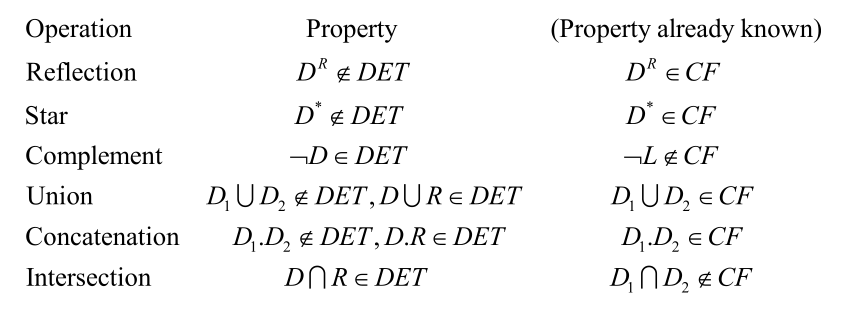
\includegraphics[width = \textwidth]{./images/detClosures.png}
					\caption{Closures properties of deterministic languages}
				\end{center}
			\end{figure}
	
	\section{Parsing}
		Parsing (syntax analysis) is the procedure to estabilish if a string belongs to a certain language. A parser is an automaton that puts in place the analysis. 
		It compute the syntax trees or gives an error if it finds one.
		
		\subsubsection{Types of parsing}
			Parsers can be classified in top-down parsers and bottom-up parsers (another distinction that's totally new to CS students, uh?) to distinguish between 
			the approach to the syntax trees.
			\begin{itemize}
				\item \emph{top down} analyzers grow the tree from the root downwards towards the leaves; this means that every step of the algorithm corresponds to 
				a \emph{derivation in the grammar} so a \emph{left} $\rightarrow$ \emph{right} passage in a rule
				\item \emph{bottom up} parsers starts from the leaves of the syntax tree and reach the root; this means that every step of the parsing procedure 
				corresposnds to a \emph{reduction in the grammar}, so a \emph{right} $\rightarrow$ \emph{left} passage in a rule
			\end{itemize}
		
		\subsection{Grammars as networks of finite automata}
			To build a recognizer for a grammar, we can see it as a set of indipendent productions for each nonterminal. Every nonterminal is associated with a 
			dedicated machine (a FSA, for example) that when has to read another nonterminal just "invokes" another machine to do so.

			This means that, at the end of the transformation, we have a machine for every nonterminal, that can interpret all the productions of said nonterminal, 
			and on the arcs has all and only the right-side elements of the rule taken into account.
			
			\subsubsection{Good example}
				We consider a grammar that generates arithmetic expressions.
				\begin{figure}[htp]
					\begin{center}
						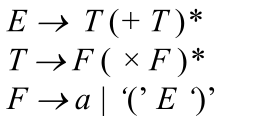
\includegraphics[]{./images/exGrammar.png}
					\end{center}
				\end{figure}
				We isolate the three nonterminals E, T and F and build a machine for each one of them
				\begin{figure}[htp]
					\begin{center}
						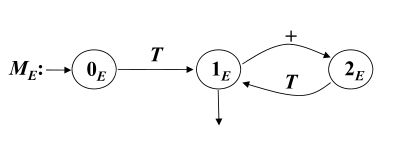
\includegraphics[]{./images/exE.png}
					\end{center}
				\end{figure}
				\begin{figure}[htp]
					\begin{center}
						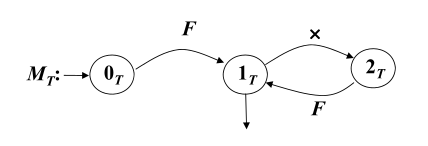
\includegraphics[]{./images/exT.png}
					\end{center}
				\end{figure}
				\begin{figure}[htp]
					\begin{center}
						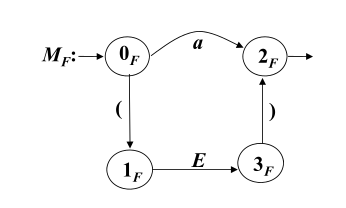
\includegraphics[]{./images/exF.png}
					\end{center}
				\end{figure}
				
		\subsection{Lookahead sets}
			All parsers are implemented as DPDA. They rely on a second component, the lexical analyzer, that reads the input stream and recognizes the patterns in it 
			in order to separate all the lexeme (or tokens) to give to the parser itself.

			To ensure the automaton is actually deterministic, parsers \emph{preprocess} the grammar's rules, and select the sets of tokens that can be read after 
			each move; these are the \emph{followers} or \emph{lookahead} set. These sets of token are useful when another machine in the network must be called: 
			it's necessary to know which character we \emph{will} read and compare it with the first character read in the machines. To be noted: each 
			\emph{nonterminal, for each configuration,} has a set of lookahead characters. 
			
			\subsubsection{Lookahead and closures}
				Each pair \{state, token\} is said to be a candidate if the token is a legal lookahed character for the current activation of the machine in state 
				"state". That does not mean so much, at the end of the day.

				To compute each set of candidates we use a \emph{closure function}. The closure function is defined this way:

				Let \emph{C} be a set of candidates:
				\begin{equation}
					\text{closure(\emph{C})} =
					\begin{cases}
				  		\text{\emph{C}} \\
				  		\langle 0_b, b \rangle \in \text{closure(\emph{C}) if }
				  		\begin{cases}
				  			\exists \text{ candidate } \langle q, a\rangle \in \text{\emph{C} \textbf{and}}\\
				  			\exists \text{ arc in the machine net so that } q \xrightarrow{B} r \text{\textbf{ and}}\\
				  			b \in \text{Ini(L(r)} \cdot a \text{)}
				  		\end{cases} 
					\end{cases}
			  	\end{equation}
			  	EXPLANATION OF THE FORMULA: the formula returns a \emph{set of candidates}, so a set of pairs $\langle$ state, character $\rangle$. Its input is 
				\emph{another set of candidates}, so the output will be the closure not of a unique state, but of a set of them. The formula states that a candidate 
				can be in the closure if:
			  	\begin{itemize}
			  		\item The candidate \emph{is} the closure;
			  		\item The candidate is composed of an initial state (in the formula written as $0_b$) of a machine in the network and a character ("b") which is 
					in the set of initials of a language that is \emph{reached through machine B}.
			  	\end{itemize}
			  	Notice how subtle the recursivity is: in order to compute a language of a state (L(r) in this case) we should build the closure of the candidates 
				starting from state r. The fixed point is reached when state r is final, so L(r) is $\epsilon$ thus the following character ("a" in the formula) is 
				added to the candidate.
			
			\subsubsection{Meaningful example}
				We consider grammar G
				\begin{equation}
					G = 
					\begin{cases}
						E \rightarrow T^\ast\\
						T \rightarrow \text{'(' } E \text{ ')' } \vert \text{ a}
					\end{cases}
				\end{equation}
				that generates expressions and terms. We consider the machine network
				\begin{figure}[H]
					\begin{center}
						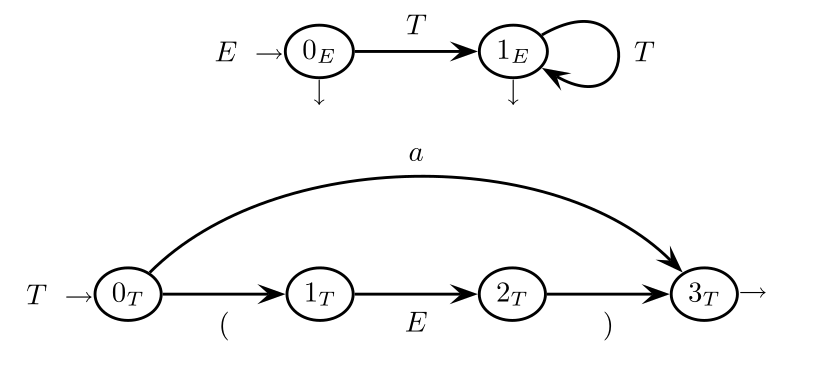
\includegraphics[width = \textwidth]{./images/exNetwork.png}
					\end{center}
				\end{figure}
				We compute the closure for candidate $\langle 0_e, \dashv \rangle$
				\begin{itemize}
					\item $\langle 0_e, \dashv \rangle$
					\item $\langle 0_t, \text{ ( }\rangle$
					\item $\langle 0_t, \text{ a }\rangle$
					\item $\langle 0_t, \dashv \rangle$
				\end{itemize}
		
		\subsection{ELR parsers}
			ELR = Extended Left to right Rightmost

			When reducing a string in input, a bottom up parser has two possible moves available: \emph{shift} to the next character (that simply means that a new 
			state is pushed on the stack and no pattern has been recognized yet) or \emph{reduce}: this means that a pattern (a right part of a rule) has been fully 
			recognized and a state can be popped from the stack. These two operations are an adapted version of the pop-push model for the memory. They also represent 
			the moving forward and backward in the rules of the grammar.

			ELR is the name for the parsers that recognize a EBNF grammar.

			To build the recognizer starting from the grammar a three-phase method has been outlined:
			\begin{enumerate}
				\item (Prerequisites: we have a network of machines that describes the grammar's rules) We build a special automaton called \emph{pilot automaton} 
				that is a generalization of the machines network. It covers all the possible combination of states and input.
				\item The pilot is inspected to check if it's suitable for deterministic parsing, and three types of failure are searched for (we'll discuss them 
				in a moment).
				\item If the test at point 2 is passed, then the DPDA is built from the pilot. 
			\end{enumerate}
			
			\subsubsection{Construction of the pilot automaton}
				The pilot automaton is (as already said) a method to represent \emph{all} the possible computational path of another one. Every state (called macro 
				state or m-state) is labeled as all the states it represents, and all the arcs keep in consideration all the possible reading for all the possible 
				states encapsulated in a single m-state.

				Every state is divided in 4 parts:
				\begin{itemize}
					\item the two (canonically) upper parts are the \emph{base} candidates: the states and lookahead characters of \textbf{non initial} state;
					\item the two (canonically) lower parts are reserved to the \emph{kernel} candidates: the states and associated lookahead of the 
					\textbf{initial} state.
				\end{itemize}
				Every final state in every m-state is usually highlighted (to help spot reductions).

				An algorithm that creates a pilot automaton can be described in this way:
				\begin{enumerate}
					\item The initial state groups the first state of the first accessed machine AND all the states of the machine that can be reached with a 
					$\epsilon$-move. (So? They're all the first states of the nonterminals that \emph{label} the outgoing arcs from the initial state. Being 
					all initial states \emph{for construction}, first m-state does not have the base part)
					\item All the other states are built in a similar way: following an arc, I add all the state that I can found to the next m-state; I select 
					the initial ones and put them in the closure, then I check for states that are reachable through a $\epsilon$-move, and also add them to the 
					closure. For the closure part, I shall recalculate the lookaheads, things that \emph{generally} I do not do with the pure base part.
				\end{enumerate}
				Is a pilot automaton still a PDA? Yes: the extra labeling of the states and the interpretation of the strings can be seen as pushing and poppoing 
				the entire candidates onto the stack and popped back when needed.
				
			\subsubsection{Meaningful example}
				We build the pilot automaton for the grammar in (5); at first glance, it can seem overly complicated, so I'll add a list of things to be noted.
				\begin{itemize}
					\item All m-states have a number of outgoing arcs that's equal to the number of outgoing arcs of \emph{all his states combined}
					\item The first state has no base part
					\item \underline{Following a path on the machine chart translates in "inheriting" the lookahead set}
					\item Watching the graph, there are two visible subsets that represents the two possible paths towards the accepting states: one in the 
					"upper level" (which has as a lookahead $\dashv$) and one in the "nested level". The first is composed of the states 
					\{$I_0$, $I_3$, $I_8$, $I_2$\} and the second one of the states \{$I_3$, $I_6$, $I_7$, $I_5$\}
				\end{itemize}
				\begin{figure}[H]
					\begin{center}
						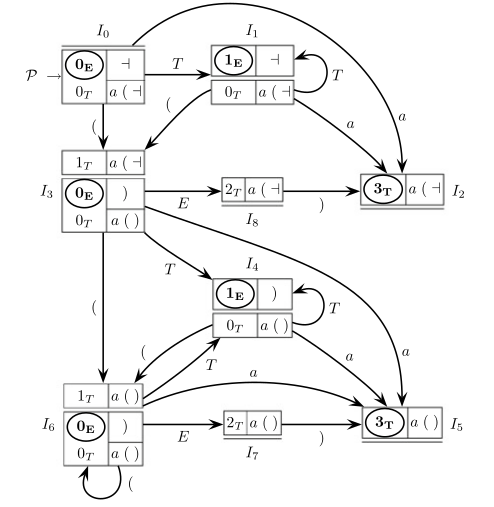
\includegraphics[]{./images/pilotAutomaton.png}
					\end{center}
				\end{figure}
				
			\subsubsection{Another meaningful example}
				Without forgetting we are at the \emph{first} step of our DPDA building, I add another good example.

				We start from this machine sets:
				\begin{figure}[H]
					\begin{center}
						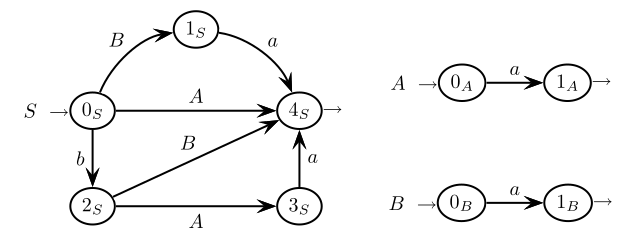
\includegraphics[width = \textwidth]{./images/ex2.png}
					\end{center}
				\end{figure}
				We derive the pilot automaton with the algorithm described above:
				\begin{figure}[H]
					\begin{center}
						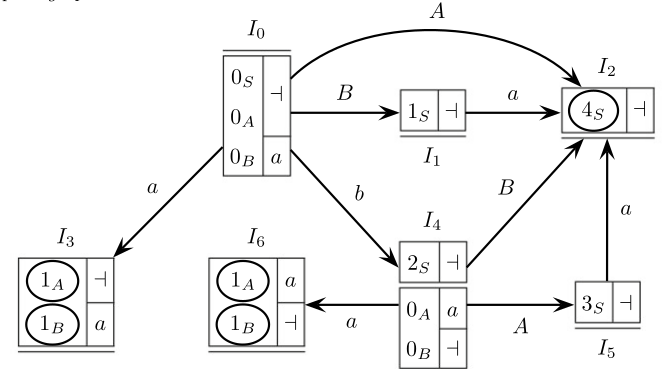
\includegraphics[width = \textwidth]{./images/ex2Pilot.png}
					\end{center}
				\end{figure}
				Again, I add a short list of things to be noted
				\begin{itemize}
					\item the first transition labeled "a" is the perfect example of \emph{following a paht makes you inherit lookaheads};
					\item m-states $I_3$ and $I_6$ represents the same states, but with different lookaheads;
				\end{itemize}
				
			\subsubsection{Deterministic check (also called ELR condition)}	
				The three possible failures in deterministic check:
				\begin{itemize}
					\item shift reduce conflicts: both a shift and a reduce are a possible in a certain configuration. This means that in a pilot automaton for all 
					the candidates $\langle q, \pi \rangle \in I$ so that q is final and for all the arcs $I \xrightarrow{a} I'$ that go out from I with terminal 
					label a it must hold that $a \notin \pi$;
					\item reduce reduce conflicts: two possible (or more) reduce paths are possible in a given configuration. In a pilot automaton, it's formulated 
					as: for all the candidate $\langle q, \pi \rangle, \langle r, \rho \rangle \in I$ that q and r are both final it must hold that 
					$\pi \cap \rho = \emptyset$;
					\item convergence conflicts: two different computations share a lookahead and a future state (this could cause reducing conflicts). This conflict 
					is the most tricky to discover, as it can only be done analyzing the graph manually: the condition to be met is something like "no different 
					states in a single m-state share a lookahead and a state".
				\end{itemize}
				
			\subsubsection{Parser algorithm}
				We focus on the implementation that makes use of a vector stack, so a LIFO memory with has also and index-like access (like vectors. You should guess 
				what a vector stack is). This enables the parser to save the exact position to return to when a reduce move is performed, accessing directly the cell 
				pointed with the saved index.

				The accepting procedure is quite obvious: the pilot automaton is traversed following the arcs when a new term is read, and reducing when the next term 
				is equal to the lookahead char in the m-state. Accepting is when we reach a final state and we only have the axiom on the stack. This procedure is an 
				incremental process: every time a m-state is leaved, on the stack are pushed all the possible candidates, and the next m-state will save the pointer 
				(index) to the previous one and so on, so that at reduce time the parser can pop off all the states from the stacks just following the indexes.

				(The official and formal way to describe the algorithm is leaved to the curious reader: page 271+ of the "Formal languages and Compilation" book from 
				Reghizzi, Breveglieri, Morzenti)
		
		\subsection{ELR parser re written}
		This question is exercise $3$ in the exam.
			ELL and ELR are two different methods to build parsers.
			Let's analyse ELR starting from an example:
			\begin{figure}[H]
				\centering
                \subfloat[][\emph{Machine A}]{
					\begin{tikzpicture}[>=stealth',shorten >=1pt,auto,node distance=2cm]
						\node[] (initial) {$A$};
						\node[state] (0a) [right of =initial]      {$0_A$};
						\node[state]         (1a) [right of=0a]  {$1_A$};
						\node[] (final)[right of =1a]{};
						
						\path[->](initial) edge node {} (0a);
						\path[->]          (0a)  edge node {c} (1a);
						\path[->]          (1a)  edge node {} (final);
					\end{tikzpicture}
					\label{fig:A}
				} \\
                \subfloat[][\emph{Axiom $S$}]{
					\resizebox{0.9\textwidth}{!}{
						\begin{tikzpicture}[>=stealth',shorten >=1pt,auto,node distance=2cm]
							\node[] (initial) {$S$};
							\node[state] (0s) [right of =initial]      {$0_S$};
							\node[state]         (1s) [right of=0s]  {$1_S$};
							\node[state]         (2s) [right of=1s]  {$2_S$};
							\node[state]         (3s) [right of=2s]  {$3_S$};
							\node[state]         (4s) [right of=3s]  {$4_S$};
							\node[] (final)[right of =4s]{};
							
							\path[->](initial) edge node {} (0a);
							\path[->]          (0s)  edge node {a} (1s);
							\path[->]          (1s)  edge node {a} (2s);
							\path[->]          (2s)  edge node {b} (3s);
							\path[->]          (3s)  edge node {c} (4s);
							\path[->]          (4s)  edge node {} (final);
							\path[->][in=45,out=135]          (3s)  edge node [swap ]{$A$} (1s);
							\path[->][in=-45,out=-135]          (4s)  edge node {$C$} (2s);
						\end{tikzpicture}
					}
					\label{fig:B}
				}\\
				\subfloat[][\emph{Machine C}]{
					\begin{tikzpicture}[>=stealth',shorten >=1pt,auto,node distance=2cm]
						\node[] (initial) {$C$};
						\node[state] (0c) [right of =initial]      {$0_C$};
						\node[state]         (1c) [right of=0c]  {$1_C$};
						\node[state]         (2c) [right of=1c]  {$2_C$};
						\node[] (final)[right of =2c]{};
						
						\path[->](initial) edge node {} (0a);
						\path[->]          (0c)  edge node {d} (1c);
						\path[->]          (2c)  edge node {} (final);
						\path[->][in=45,out=135]          (2c)  edge node [swap ]{$A$} (1c);
						\path[->][in=-135,out=-45]          (1c)  edge node {$a$} (2c);
					\end{tikzpicture}
					\label{fig:C}
				}
                \caption{Example}
                \label{fig:mainexample}
			\end{figure}
			ELR: tries to completely match one machine to the prefix it finds. If it recognizes it, one of these three nonterminal symbols is attributed to it.
			\begin{definition}[Reduction]
				The production substitutes the expansion of the production with the symbol of the rule
			\end{definition}
			We want to perform reductions until we are left with only one symbol: the one of the axiom (considering figure \ref{fig:mainexample}, $S$): at that point 
			we have recognized a string.

			We will see the algorithm in a momnent, after some critical points we need to clarify: at the first stwp we want to create the initial state of the pilot 
			automaton. How? we want to compute the closure of the initial state of the axiom.
			\begin{definition}[Closure]
				Is the set of all the candidates that can be found from a given state and the lookahead.
			\end{definition}
			Let's dig more into this definition, looking at what is a \textbf{candidate} and the \textbf{lookahead} in an informal way.

			ELR wants to find the longest prefix: the candidate basically tells to the algorithm ``\emph{I think that at this point we will possibly recognize in
			the end one of these three machines}''. After recognizing one of the production (say $A$ or $C$ in the example), there must be an additional character.
			This is the secret sauce of ELR algorithm, and is what ives us the certainty (if we are in ELR1 case, we will see what this mean) that we are not 
			doing a false match. For example: $c$ can appear inside $s$, or can be the entire tree production of $A$. How do we distinguish this case?
			\begin{itemize}
				\item To recognize $A$ (i.e., if $c$ comes from $A$, figure \ref{fig:A}), we must find for example $a$ coming from 
				$1_S\overset{a}{\longrightarrow}2_S$ after character in $A$, because we can 
				only recognize $A$ taking the arc $3_S\overset{A}{\longrightarrow}1_S$. In this case, $a$ coming from $1_S\overset{a}{\longrightarrow}2_S$ is the 
				\textbf{lookahead} (the character that comes \emph{after} having recognized $A$), which gives the certainty that we recognized $A$.
				\item If the $c$ instead came from $3_S\overset{c}{\longrightarrow}4_S$ (figure \ref{fig:B}), after that we have the production $C$, and its first 
				character is $d$ ($0_C\overset{d}{\longrightarrow}1_C$), which is different from $a$.
			\end{itemize}
			So, when we arrive in $3_S$ (fig \ref{fig:B}), we have two candidates:
			\begin{enumerate}
				\item $3_S\longrightarrow 4S$ in which we continue recognizing the production $S$.
				\item $3_S\longrightarrow 0A$ in which we start recognizing the production $A$.
			\end{enumerate}
			ELR looks at all these possible candidates in parallel. Until we read the $c$ and the lookahead, we don't know which is the option in which we are: 
			we need to bring on all the possible options until we find the correct lookahead (at that point we have found the correct candidate tha we need to 
			continue parsing the string).

			Candidates are tuples:
			\begin{equation*}
				C=\langle q,r\rangle
			\end{equation*}
			where:
			\begin{itemize}
				\item $q$: A machine of the state;
				\item $r$: $\Sigma$, where $\Sigma$ is the alphabet, (while $V$ are the nonterminals, hot present here).
			\end{itemize}
			In every state of ELR, we have these states (separate from states of the machine of the production), which are called \emph{macro states}, or 
			\emph{m-states}.
			
			In each state of the pilot we have a set of candidates: the transitions of ELR recognizes all the set of characters in the alphabet and the 
			nonterminals, becausr when we replace production with nonterminal symbols, is what the pilot need to be able to do: replace the production with the 
			correct nonterminal symbol.

			Let's see how we build transitions and symbols:
			Initial state is built from all the initial candidates that can be found at the beginning of the string. Since we are at the beginning of the 
			string, at the end, the look ahead will be defined by at least $\dashv$ ($4_S\longrightarrow$), because when we will recognize $S$, at the end of $S$,
			when we have finished recognizing the whole string, we have the terminal character. In some cases additionally we will have some transition that 
			from the initial state of the axiom enters another machine: in that case we will have multiple lookaheads. The initial state will contain the closure 
			of $0_S$ and $\dashv$ ($\langle 0_S,\dashv\rangle$). In order to build the closure of a state we have to control all transition outgoing from $0_S$ in 
			this case. The candidates we have next, will depend from the state we are in.

			In this case, at the beginning we are in $0_S$, and the terminal character (we do not have extra candidates that need to be added).
			At the beginning we have just $0_S,\dashv$ at the beginning, and we add this new state inside the 
			ELR pilot machine. Le'ts see the two section of a node in ELR:
			\begin{itemize}
				\item \emph{base set}: elements from the closure that still belong to the original machine (in this case $S$);
				\item \emph{closure set}: contains elements of the closurethat belongs to a new machine
			\end{itemize}
			We are starting, we do not have another state, we started from nothing, hence everything goes in closure set:
			\begin{figure}[H]
				\centering
				\begin{tikzpicture}[>=stealth',shorten >=1pt,auto,node distance=2cm]
					\node (initial) [shape=rectangle,] {
						\begin{tabular}{|cc|} \toprule
							\hline
							$0_s$ & $\dashv$\\
							\hline
						\end{tabular}
						};
				\end{tikzpicture}
			\end{figure}
			In the slides, when we see \emph{closure(C)}, we don't mean only the closure set, but the entire closure!
			Now let's go on to produce the next state. Now, we need to look at all characters in the alphabet and all the nonterminals, 
			and we need to check if there is a transition from one of the states that appears in the various candidates, so for example, 
			in this case just $0_S$. For each character in the set $abcsASC$, if there is a transition that recognizes one of 
			those character from one or multiple of the states in the candidates, then we add a new transition to a new state inside the pilot.
			From $0_S,\dashv$, we have one single transition towards $1_S$ with $a$. We draw an arrow in the pilot, and the next state 
			is produced from the closure of the next state that we are going to from the next state in the $S$ machine. We were starting from $0_S,\dashv$:
			now we need to compute the closure of $\langle 1_S,\dashv\rangle$. How did we arrive to $\langle 1_S,\dashv\rangle$? we follow the transition 
			that in machine $S$ brought us to $1_S$ through $a$, and we change the state in the candidate from the initial to the final state.

			The closure of something is defined as our initial candidate itself ($1_s,\dashv$), and look at all possible transitions that from $1_S$ 
			bring us to another state, but only through one of the nonterminal symbols. The only transition does not take a nonterminal symbol. There is nothing 
			else to add in the closure, and we have finished. The building of the state is complete.
			We need now to finalize the state: what there will be in the base set? all the closure copied from the closure. we have computed the closure of 
			$1_S,\dashv$: since the closure is equal to $1_S,\dashv$ (is the closure of itself), is the base set. Then we add the closure set (new parts of new machines),
			which is empty (just put an horizontal line.)
			\begin{figure}[H]
				\centering
				\begin{tikzpicture}[>=stealth',shorten >=1pt,auto,node distance=2cm]
					\node (initial) [shape=rectangle,] {
						\begin{tabular}{|cc|} \hline
							\hline
							$0_s$ & $\dashv$\\
							\hline
						\end{tabular}
					};
					\node (first) [shape=rectangle,] [right of = initial] {
						\begin{tabular}{|cc|} \hline
							$1_s$ & $\dashv$\\
							\hline
							\hline
						\end{tabular}
					};

					\path[->](initial) edge node {a} (first);
				\end{tikzpicture}
			\end{figure}
			And we go on. we have finished with the first state ($0_S$), we have looked at all transition from initial states to all candidates, and we 
			will mark the state as completed (we'll never touch it again):
			\begin{figure}[H]
				\centering
				\begin{tikzpicture}[>=stealth',shorten >=1pt,auto,node distance=2cm]
					\node (initial) [shape=rectangle,fill=green] {
						\begin{tabular}{|cc|} \hline
							\hline
							$0_s$ & $\dashv$\\
							\hline
						\end{tabular}
					};
					\node (first) [shape=rectangle,] [right of = initial] {
						\begin{tabular}{|cc|} \hline
							$1_s$ & $\dashv$\\
							\hline
							\hline
						\end{tabular}
					};

					\path[->](initial) edge node {a} (first);
				\end{tikzpicture}
			\end{figure}
			And consider the candidate $1_S,\dashv$. From $1_S$, we have only one transition which reads $a$: we don't have to compute the closure of $1_S,\dashv$, 
			but of $2_S,\dashv$. Do we have additional production we can reach from $2_S$. We don't have a transition that recognizes a new symbol, hence we don't have
			anything to add to the closure set.:
			\begin{figure}[H]
				\centering
				\begin{tikzpicture}[>=stealth',shorten >=1pt,auto,node distance=2cm]
					\node (initial) [shape=rectangle,fill=green] {
						\begin{tabular}{|cc|} \hline
							\hline
							$0_S$ & $\dashv$\\
							\hline
						\end{tabular}
					};
					\node (first) [shape=rectangle,] [right of = initial] {
						\begin{tabular}{|cc|} \hline
							$1_S$ & $\dashv$\\
							\hline
							\hline
						\end{tabular}
					};
					\node (second) [shape=rectangle] [right of = first]{
						\begin{tabular}{|cc|}
							\hline
							$2_S$ & $\dashv$\\
							\hline
							\hline
						\end{tabular}
					};

					\path[->](initial) edge node {a} (first);
					\path[->](first) edge node {a} (second);
				\end{tikzpicture}
			\end{figure}
			Let's go on from $2_S$. Same situation. We can reach $3_S$ by reading $b$, and there is no other transition:
			\begin{figure}[H]
				\centering
				\begin{tikzpicture}[>=stealth',shorten >=1pt,auto,node distance=2cm]
					\node (initial) [shape=rectangle,fill=green] {
						\begin{tabular}{|cc|} \hline
							\hline
							$0_S$ & $\dashv$\\
							\hline
						\end{tabular}
					};
					\node (first) [shape=rectangle,] [right of = initial] {
						\begin{tabular}{|cc|} \hline
							$1_S$ & $\dashv$\\
							\hline
							\hline
						\end{tabular}
					};
					\node (second) [shape=rectangle] [right of = first]{
						\begin{tabular}{|cc|}
							\hline
							$2_S$ & $\dashv$\\
							\hline
							\hline
						\end{tabular}
					};
					\node (third) [shape=rectangle] [right of = second]{
						\begin{tabular}{|cc|}
							\hline
							$3_S$ & $\dashv$\\
							\hline
							\hline
						\end{tabular}
					};

					\path[->](initial) edge node {a} (first);
					\path[->](first) edge node {a} (second);
					\path[->](second) edge node {b} (third);
				\end{tikzpicture}
			\end{figure}
			In slides, $\delta$ , it takes one candidate, and it computes the candidates that follows a certain symbol:
			\begin{equation*}
				\delta(\langle 0_S,\dashv\rangle)=\langle 1_S,\dashv\rangle
			\end{equation*}
			We just replace the state.
			Now, in $3_S$ we have a transition that goes to a new nonterminal symbol: $3_S\overset{A}{\longrightarrow}1_S$.
			We are computing the closure of $3_S$, and we go to another state in the machine by recognizing the nonterminal symbol, 
			we need to add a new candidate in the closure set: it's not the state $1_S$, is the initial state of the machine we are 
			recognizing the nonterminal of, $A$, hence we add $0_A$, and the lookahead will be the character (or the set of characters) 
			that come after $A$ in the original machine. Here, after recognizing $A$, in $S$ we find $a$: this is our lookahead:
			\begin{figure}[H]
				\centering
				\begin{tikzpicture}[>=stealth',shorten >=1pt,auto,node distance=2cm]
					\node (initial) [shape=rectangle,fill=green] {
						\begin{tabular}{|cc|} \hline
							\hline
							$0_S$ & $\dashv$\\
							\hline
						\end{tabular}
					};
					\node (first) [shape=rectangle,] [right of = initial] {
						\begin{tabular}{|cc|} \hline
							$1_S$ & $\dashv$\\
							\hline
							\hline
						\end{tabular}
					};
					\node (second) [shape=rectangle] [right of = first]{
						\begin{tabular}{|cc|}
							\hline
							$2_S$ & $\dashv$\\
							\hline
							\hline
						\end{tabular}
					};
					\node (third) [shape=rectangle] [right of = second]{
						\begin{tabular}{|cc|}
							\hline
							$3_S$ & $\dashv$\\
							\hline
							\hline
							$0_A$ & $a$\\
							\hline
						\end{tabular}
					};

					\path[->](initial) edge node {a} (first);
					\path[->](first) edge node {a} (second);
					\path[->](second) edge node {b} (third);
				\end{tikzpicture}
			\end{figure}
			This is the important part. If we have a nonterminal between $1_S$ and $2_S$, we can't write $a$ in the closure, 
			we need to go into the machine of that nonterminal, and check the character in that machine. If there is still a 
			nonterminal character, go ahead until you find a nonterminal character.

			Let's finish computing the set of candidates: when we add a new candidate as in this case ($0_A$), we have to 
			recursively check if this adds new candidates. This does not happens: it has not transitions to nonterminal symbols, 
			but it might happen. we have finished building the closure, we need to produce the new states and transitions. Look at 
			all states, and look what is recognized. Both $0_A$ and $3_S$ recognize $c$. Add a single arc that corresponds to $c$.
			At this point, advance all the candidates where we have a recognition from the initial state of $c$, not all candidates in general.
			Only look at the ones that whose state is a state that can recognize $c$ with an outgoing transition. Advance both $3_S$ and $4_S$.
			From $3_S$ we go to $4_S$ (keep the same lookahead), and with $0_A$ we go to $1_A$, bringing forward lookahead ($a$), and this is the 
			base set:
			\begin{figure}[H]
				\centering
				\begin{tikzpicture}[>=stealth',shorten >=1pt,auto,node distance=2cm]
					\node (initial) [shape=rectangle,fill=green] {
						\begin{tabular}{|cc|} \hline
							\hline
							$0_S$ & $\dashv$\\
							\hline
						\end{tabular}
					};
					\node (first) [shape=rectangle,] [right of = initial] {
						\begin{tabular}{|cc|} \hline
							$1_S$ & $\dashv$\\
							\hline
							\hline
						\end{tabular}
					};
					\node (second) [shape=rectangle] [right of = first]{
						\begin{tabular}{|cc|}
							\hline
							$2_S$ & $\dashv$\\
							\hline
							\hline
						\end{tabular}
					};
					\node (third) [shape=rectangle] [right of = second]{
						\begin{tabular}{|cc|}
							\hline
							$3_S$ & $\dashv$\\
							\hline
							\hline
							$0_A$ & $a$\\
							\hline
						\end{tabular}
					};
					\node (fourht) [shape=rectangle] [below of = third]{
						\begin{tabular}{|cc|}
							\hline
							$4_S$ & $\dashv$\\
							$1_A$ & $a$\\
							\hline
							\hline
						\end{tabular}
					};

					\path[->](initial) edge node {a} (first);
					\path[->](first) edge node {a} (second);
					\path[->](second) edge node {b} (third);
					\path[->](third) edge node {c} (fourht);
				\end{tikzpicture}
			\end{figure}
			Let's now check if one of these two new states have a transition that recognizes a nonterminal. $1_A$ is a final state 
			(no other transitions from there), from $4_S$ we have a transition that recognizes $C$:
			\begin{figure}[H]
				\centering
				\begin{tikzpicture}[>=stealth',shorten >=1pt,auto,node distance=2cm]
					\node (initial) [shape=rectangle,fill=green] {
						\begin{tabular}{|cc|} \hline
							\hline
							$0_S$ & $\dashv$\\
							\hline
						\end{tabular}
					};
					\node (first) [shape=rectangle,] [right of = initial] {
						\begin{tabular}{|cc|} \hline
							$1_S$ & $\dashv$\\
							\hline
							\hline
						\end{tabular}
					};
					\node (second) [shape=rectangle] [right of = first]{
						\begin{tabular}{|cc|}
							\hline
							$2_S$ & $\dashv$\\
							\hline
							\hline
						\end{tabular}
					};
					\node (third) [shape=rectangle] [right of = second]{
						\begin{tabular}{|cc|}
							\hline
							$3_S$ & $\dashv$\\
							\hline
							\hline
							$0_A$ & $a$\\
							\hline
						\end{tabular}
					};
					\node (fourht) [shape=rectangle] [below of = third]{
						\begin{tabular}{|cc|}
							\hline
							$4_S$ & $\dashv$\\
							$1_A$ & $a$\\
							\hline
							\hline
							$0_C$ & $b$\\
							\hline
						\end{tabular}
					};

					\path[->](initial) edge node {a} (first);
					\path[->](first) edge node {a} (second);
					\path[->](second) edge node {b} (third);
					\path[->](third) edge node {c} (fourht);
				\end{tikzpicture}
			\end{figure}
			The closure as we notice is just $b$, $2_S$ has no other transitions or recursion. But, we have also a transition from $3_S$, in 
			which we can recognize $A$ (other than one with $c$): These transitions with nonterminals, are not different, count as the transitions with 
			terminals: we need to add these transitions also in the pilot graph. Let's build the new state in this case: we need to bring 
			ahead candidates that recognizes $A$, in this case just $3_S,\dashv$. We go to $1_S$, the state of the new candidate (with the same lookahead). Look 
			at the closure of this state: from $1_S$, we have no transitions that goes to another state through a nonterminal: this state is finished here:
			\begin{figure}[H]
				\centering
				\begin{tikzpicture}[>=stealth',shorten >=1pt,auto,node distance=2cm]
					\node (initial) [shape=rectangle,fill=green] {
						\begin{tabular}{|cc|} \hline
							\hline
							$0_S$ & $\dashv$\\
							\hline
						\end{tabular}
					};
					\node (first) [shape=rectangle,] [right of = initial] {
						\begin{tabular}{|cc|} \hline
							$1_S$ & $\dashv$\\
							\hline
							\hline
						\end{tabular}
					};
					\node (second) [shape=rectangle] [right of = first]{
						\begin{tabular}{|cc|}
							\hline
							$2_S$ & $\dashv$\\
							\hline
							\hline
						\end{tabular}
					};
					\node (third) [shape=rectangle] [right of = second]{
						\begin{tabular}{|cc|}
							\hline
							$3_S$ & $\dashv$\\
							\hline
							\hline
							$0_A$ & $a$\\
							\hline
						\end{tabular}
					};
					\node (fourht) [shape=rectangle] [below of = third]{
						\begin{tabular}{|cc|}
							\hline
							$4_S$ & $\dashv$\\
							$1_A$ & $a$\\
							\hline
							\hline
							$0_C$ & $b$\\
							\hline
						\end{tabular}
					};
					\node (fifth) [shape=rectangle] [below of = second]{
						\begin{tabular}{|cc|}
							\hline
							$1_S$ & $\dashv$\\
							\hline
							\hline
						\end{tabular}
					};

					\path[->](initial) edge node {a} (first);
					\path[->](first) edge node {a} (second);
					\path[->](second) edge node {b} (third);
					\path[->](third) edge node {c} (fourht);
					\path[->](third) edge node [swap] {A} (fifth);
				\end{tikzpicture}
			\end{figure}
			When we build a new state identical, with all set of candidates, as another state (the highlighted ones):
			\begin{figure}[H]
				\centering
				\begin{tikzpicture}[>=stealth',shorten >=1pt,auto,node distance=2cm]
					\node (initial) [shape=rectangle,fill=green] {
						\begin{tabular}{|cc|} \hline
							\hline
							$0_S$ & $\dashv$\\
							\hline
						\end{tabular}
					};
					\node (first) [shape=rectangle,] [right of = initial, fill=red] {
						\begin{tabular}{|cc|} \hline
							$1_S$ & $\dashv$\\
							\hline
							\hline
						\end{tabular}
					};
					\node (second) [shape=rectangle] [right of = first]{
						\begin{tabular}{|cc|}
							\hline
							$2_S$ & $\dashv$\\
							\hline
							\hline
						\end{tabular}
					};
					\node (third) [shape=rectangle] [right of = second]{
						\begin{tabular}{|cc|}
							\hline
							$3_S$ & $\dashv$\\
							\hline
							\hline
							$0_A$ & $a$\\
							\hline
						\end{tabular}
					};
					\node (fourht) [shape=rectangle] [below of = third]{
						\begin{tabular}{|cc|}
							\hline
							$4_S$ & $\dashv$\\
							$1_A$ & $a$\\
							\hline
							\hline
							$0_C$ & $b$\\
							\hline
						\end{tabular}
					};
					\node (fifth) [shape=rectangle] [below of = second,fill=red]{
						\begin{tabular}{|cc|}
							\hline
							$1_S$ & $\dashv$\\
							\hline
							\hline
						\end{tabular}
					};

					\path[->](initial) edge node {a} (first);
					\path[->](first) edge node {a} (second);
					\path[->](second) edge node {b} (third);
					\path[->](third) edge node {c} (fourht);
					\path[->](third) edge node [swap] {A} (fifth);
				\end{tikzpicture}
			\end{figure}
			This means, that they are the \textbf{same} state, they are not different: we can never have two identical states (same set 
			of candidates). Hence, we did not need the last node:
			\begin{figure}[H]
				\centering
				\begin{tikzpicture}[>=stealth',shorten >=1pt,auto,node distance=2cm]
					\node (initial) [shape=rectangle,fill=green] {
						\begin{tabular}{|cc|} \hline
							\hline
							$0_S$ & $\dashv$\\
							\hline
						\end{tabular}
					};
					\node (first) [shape=rectangle] [right of = initial] {
						\begin{tabular}{|cc|} \hline
							$1_S$ & $\dashv$\\
							\hline
							\hline
						\end{tabular}
					};
					\node (second) [shape=rectangle] [right of = first]{
						\begin{tabular}{|cc|}
							\hline
							$2_S$ & $\dashv$\\
							\hline
							\hline
						\end{tabular}
					};
					\node (third) [shape=rectangle] [right of = second]{
						\begin{tabular}{|cc|}
							\hline
							$3_S$ & $\dashv$\\
							\hline
							\hline
							$0_A$ & $a$\\
							\hline
						\end{tabular}
					};
					\node (fourht) [shape=rectangle] [below of = third]{
						\begin{tabular}{|cc|}
							\hline
							$4_S$ & $\dashv$\\
							$1_A$ & $a$\\
							\hline
							\hline
							$0_C$ & $b$\\
							\hline
						\end{tabular}
					};

					\path[->](initial) edge node {a} (first);
					\path[->](first) edge node {a} (second);
					\path[->](second) edge node {b} (third);
					\path[->](third) edge node {c} (fourht);
					\path[->](third) edge [in=-45, out=-135] node [swap] {A} (first);
				\end{tikzpicture}
			\end{figure}
			Be careful, always try to build closure: maybe state is not the same. Pay attention in sayng ``yes, it is duplicate''.
			Mark now the completion of the states:
			\begin{figure}[H]
				\centering
				\begin{tikzpicture}[>=stealth',shorten >=1pt,auto,node distance=2cm]
					\node (initial) [shape=rectangle,fill=green] {
						\begin{tabular}{|cc|} \hline
							\hline
							$0_S$ & $\dashv$\\
							\hline
						\end{tabular}
					};
					\node (first) [shape=rectangle,fill=green] [right of = initial] {
						\begin{tabular}{|cc|} \hline
							$1_S$ & $\dashv$\\
							\hline
							\hline
						\end{tabular}
					};
					\node (second) [shape=rectangle,fill=green] [right of = first]{
						\begin{tabular}{|cc|}
							\hline
							$2_S$ & $\dashv$\\
							\hline
							\hline
						\end{tabular}
					};
					\node (third) [shape=rectangle,fill=green] [right of = second]{
						\begin{tabular}{|cc|}
							\hline
							$3_S$ & $\dashv$\\
							\hline
							\hline
							$0_A$ & $a$\\
							\hline
						\end{tabular}
					};
					\node (fourht) [shape=rectangle] [below of = third]{
						\begin{tabular}{|cc|}
							\hline
							$4_S$ & $\dashv$\\
							$1_A$ & $a$\\
							\hline
							\hline
							$0_C$ & $b$\\
							\hline
						\end{tabular}
					};

					\path[->](initial) edge node {a} (first);
					\path[->](first) edge node {a} (second);
					\path[->](second) edge node {b} (third);
					\path[->](third) edge node {c} (fourht);
					\path[->](third) edge [in=-45, out=-135] node [swap] {A} (first);
				\end{tikzpicture}
			\end{figure}
			We need to go on with the fourth state, which has four candidates. Let's look at what becomes.
			\begin{itemize}
				\item From $4_S$ we can recognize $C$, or it is a final state.
				\item From $1_A$ we have finished parsing.
				\item From $0_C$ we can recognize $d$.
			\end{itemize}
			We have found two final states, $4_S$ and $1_A$. circle the final states for exam (just an additional thing, not necessary for ELR).
			\begin{figure}[H]
				\centering
				\begin{tikzpicture}[>=stealth',shorten >=1pt,auto,node distance=2cm]
					\node (initial) [shape=rectangle,fill=green] {
						\begin{tabular}{|cc|} \hline
							\hline
							$0_S$ & $\dashv$\\
							\hline
						\end{tabular}
					};
					\node (first) [shape=rectangle,fill=green] [right of = initial] {
						\begin{tabular}{|cc|} \hline
							$1_S$ & $\dashv$\\
							\hline
							\hline
						\end{tabular}
					};
					\node (second) [shape=rectangle,fill=green] [right of = first]{
						\begin{tabular}{|cc|}
							\hline
							$2_S$ & $\dashv$\\
							\hline
							\hline
						\end{tabular}
					};
					\node (third) [shape=rectangle,fill=green] [right of = second]{
						\begin{tabular}{|cc|}
							\hline
							$3_S$ & $\dashv$\\
							\hline
							\hline
							$0_A$ & $a$\\
							\hline
						\end{tabular}
					};
					\node (fourht) [shape=rectangle] [below of = third]{
						\begin{tabular}{|cc|}
							\hline
							\circled{$4_S$} & $\dashv$\\
							\circled{$1_A$} & $a$\\
							\hline
							\hline
							$0_C$ & $b$\\
							\hline
						\end{tabular}
					};

					\path[->](initial) edge node {a} (first);
					\path[->](first) edge node {a} (second);
					\path[->](second) edge node {b} (third);
					\path[->](third) edge node {c} (fourht);
					\path[->](third) edge [in=-45, out=-135] node [swap] {A} (first);
				\end{tikzpicture}
			\end{figure}
			We need to go on with the fourth state, which has four candidates. Let's look at what becomes.
			\begin{itemize}
				\item From $4_S$ we can recognize $C$, or it is a final state.
				\item From $1_A$ we have finished parsing.
				\item From $0_C$ we can recognize $d$.
			\end{itemize}
			Anyway, we can start seing a pattern:
			\begin{enumerate}
				\item Consider all candidates (base or closure set)
				\item Follow each transition on the machines
				\item See in which state you go (copying lookahead when you stay in the same machine)
				\item Compute the closure if one of those in the base set has a Nonterminal after, and put in the closure set.
			\end{enumerate}
			Let's go on. Because from $4_S$ we can also read $C$: we need to add another arc which recognizes $C$. We are going from $2_S$, in which 
			we have already seen that we can only go to $3_S$ by reading $b$ (closure set empty), we don't have other transition that goes to a 
			non terminal state. We already have a state with the candidate $2_S,\dashv$:
			\begin{figure}[H]
				\centering
				\begin{tikzpicture}[>=stealth',shorten >=1pt,auto,node distance=2cm]
					\node (initial) [shape=rectangle,fill=green] {
						\begin{tabular}{|cc|} \hline
							\hline
							$0_S$ & $\dashv$\\
							\hline
						\end{tabular}
					};
					\node (first) [shape=rectangle,fill=green] [right of = initial] {
						\begin{tabular}{|cc|} \hline
							$1_S$ & $\dashv$\\
							\hline
							\hline
						\end{tabular}
					};
					\node (second) [shape=rectangle,fill=green] [right of = first]{
						\begin{tabular}{|cc|}
							\hline
							$2_S$ & $\dashv$\\
							\hline
							\hline
						\end{tabular}
					};
					\node (third) [shape=rectangle,fill=green] [right of = second]{
						\begin{tabular}{|cc|}
							\hline
							$3_S$ & $\dashv$\\
							\hline
							\hline
							$0_A$ & $a$\\
							\hline
						\end{tabular}
					};
					\node (fourht) [shape=rectangle] [below of = third]{
						\begin{tabular}{|cc|}
							\hline
							\circled{$4_S$} & $\dashv$\\
							\circled{$1_A$} & $a$\\
							\hline
							\hline
							$0_C$ & $b$\\
							\hline
						\end{tabular}
					};

					\path[->](initial) edge node {a} (first);
					\path[->](first) edge node {a} (second);
					\path[->](second) edge node {b} (third);
					\path[->](third) edge node {c} (fourht);
					\path[->](third) edge [in=-45, out=-135] node [swap] {A} (first);
					\path[->](fourht) [in=-90, out=-135] edge node{C}(second);
				\end{tikzpicture}
			\end{figure}
			Let's look at the other candidates: $1_A$ and $0_C$: $1_A$ is a final state, but does not recognize anything else, so we do not need to do anything 
			more in order to take into account that candidate, because when we reach at that state, the next character is the one in the lookahead, and we can tell 
			if we have recognized the production $A$. From the pilot graph point of view, there is nothing else.
			From $0_C$, we can read $d$, and no other nonterminal symbols from there: we need to add a new transition to a new state which recognizes character $d$,
			and as base set that state will have the advancement of the candidate, with the same lookahead:
			\begin{figure}[H]
				\centering
				\begin{tikzpicture}[>=stealth',shorten >=1pt,auto,node distance=2cm]
					\node (initial) [shape=rectangle,fill=green] {
						\begin{tabular}{|cc|} \hline
							\hline
							$0_S$ & $\dashv$\\
							\hline
						\end{tabular}
					};
					\node (first) [shape=rectangle,fill=green] [right of = initial] {
						\begin{tabular}{|cc|} \hline
							$1_S$ & $\dashv$\\
							\hline
							\hline
						\end{tabular}
					};
					\node (second) [shape=rectangle,fill=green] [right of = first]{
						\begin{tabular}{|cc|}
							\hline
							$2_S$ & $\dashv$\\
							\hline
							\hline
						\end{tabular}
					};
					\node (third) [shape=rectangle,fill=green] [right of = second]{
						\begin{tabular}{|cc|}
							\hline
							$3_S$ & $\dashv$\\
							\hline
							\hline
							$0_A$ & $a$\\
							\hline
						\end{tabular}
					};
					\node (fourht) [shape=rectangle] [below of = third]{
						\begin{tabular}{|cc|}
							\hline
							\circled{$4_S$} & $\dashv$\\
							\circled{$1_A$} & $a$\\
							\hline
							\hline
							$0_C$ & $b$\\
							\hline
						\end{tabular}
					};
					\node (fifth) [shape=rectangle] [below of = first]{
						\begin{tabular}{|cc|}
							\hline
							$1_C$ & $b$\\
							\hline
							\hline
						\end{tabular}
					};

					\path[->](initial) edge node {a} (first);
					\path[->](first) edge node {a} (second);
					\path[->](second) edge node {b} (third);
					\path[->](third) edge node {c} (fourht);
					\path[->](third) edge [in=-45, out=-135] node [swap] {A} (first);
					\path[->](fourht) [in=-90, out=-135] edge node{C}(second);
					\path[->](fourht) edge node [swap]{d} (fifth);
				\end{tikzpicture}
			\end{figure}
			And compute the closure: we can re-enter into $S$. We need to add a new candidate in the closure set:
			\begin{figure}[H]
				\centering
				\begin{tikzpicture}[>=stealth',shorten >=1pt,auto,node distance=2cm]
					\node (initial) [shape=rectangle,fill=green] {
						\begin{tabular}{|cc|} \hline
							\hline
							$0_S$ & $\dashv$\\
							\hline
						\end{tabular}
					};
					\node (first) [shape=rectangle,fill=green] [right of = initial] {
						\begin{tabular}{|cc|} \hline
							$1_S$ & $\dashv$\\
							\hline
							\hline
						\end{tabular}
					};
					\node (second) [shape=rectangle,fill=green] [right of = first]{
						\begin{tabular}{|cc|}
							\hline
							$2_S$ & $\dashv$\\
							\hline
							\hline
						\end{tabular}
					};
					\node (third) [shape=rectangle,fill=green] [right of = second]{
						\begin{tabular}{|cc|}
							\hline
							$3_S$ & $\dashv$\\
							\hline
							\hline
							$0_A$ & $a$\\
							\hline
						\end{tabular}
					};
					\node (fourht) [shape=rectangle] [below of = third]{
						\begin{tabular}{|cc|}
							\hline
							\circled{$4_S$} & $\dashv$\\
							\circled{$1_A$} & $a$\\
							\hline
							\hline
							$0_C$ & $b$\\
							\hline
						\end{tabular}
					};
					\node (fifth) [shape=rectangle] [below of = first]{
						\begin{tabular}{|cc|}
							\hline
							$1_C$ & $b$\\
							\hline
							\hline
							$0_S$ & $b$\\
							\hline
						\end{tabular}
					};
					
					\path[->](initial) edge node {a} (first);
					\path[->](first) edge node {a} (second);
					\path[->](second) edge node {b} (third);
					\path[->](third) edge node {c} (fourht);
					\path[->](third) edge [in=-45, out=-135] node [swap] {A} (first);
					\path[->](fourht) [in=-90, out=-135] edge node{C}(second);
					\path[->](fourht) edge node [swap]{d} (fifth);
				\end{tikzpicture}
			\end{figure}
			Why the lookahead is $b$? Is the next character we can read after the transition that recognizes our nonterminal symbol. But at 
			this point, after $2_C$, the machine $C$ ends: the character we read, is the same lookahead by recognizing $C$: we will have the lookahead that 
			we had before with $C$. This because when $S$ ends in $2_C$, also $C$ ends, so the lookahead is the same.
			
			N.B.: we did not added the $\dashv$! because 
			is just the production of $C$ that ended, the terminal character is only at the end of the final string, not at the end of every machine (production), because 
			this would result in $\dashv$ inside of the string.

			And you have to go on like this. % if necessary other things, resume from 1:01:51 of lesson of professor Daniele Cattaneo, 20221110
		\subsection{ELL parsers}
			ELL = Extended Left to right Leftmost

			ELL parsers are among the most basic top down parsers; the idea is to mimic the traversing of the machines network. The string is 
			\emph{progressively generated} using the grammar rules character by character until $\dashv$ is reached. ELL parsers relies on a stronger assumption 
			than ELRs: so that the input string can identify the rule that produces it \emph{starting from the first character}.

			The most used technique is to enrich the arcs of the pilot automaton with "guide sets" that communicate the next characters that can be encountered. 
			Relying on a stronger hypothesis means being effective in fewer cases: ELL parsers can't be built if
			\begin{itemize}
				\item Multiple transitions between states are defined. This simply means that ELL parsing isn't applicable to \emph{all} the pilot automata where 
				two or more states in the same m-state originate an arc with the same label;
				\item There are left-recursive derivation;
				\item The pilot automaton does not meet ELR condition (ELL represents a smaller set of languages). 
			\end{itemize}
			These three conditon form the \textbf{ELL condition} for automata.
			
			\subsubsection{Parser Control Flow Graph}
				A PCFG is a representation of the automata that compose the machine network that \emph{links} them all together, highlighting subsequent calls 
				and recursive dependencies. From the PCFG it's easy to derive directly the parser code.

				Starting from the machine net graph, building a PCFG means:
				\begin{enumerate}
					\item adding call arcs: these arcs connect the states that have an outgoing arc labeled as nonterminal with the first state of the machine that 
					recognizes that nonterminal;
					\item labeling call arcs: every call arc is enriched with a set of nonterminals that are the "guide set" for that call. This set of nonterminals 
					is composed of all the followers of that call:
						\begin{itemize}
							\item token that are the initials of the language generated by the submachine
							\item the empty string if the language of the subm is nullable
							\item the nonterminals that labels the subsubcalls to other submachines
						\end{itemize}
					\item enriching final states with so-called "prospect sets": prospect sets are the union of \emph{all} lookahead sets of \emph{all} the 
					occurrence of that state in the pilt automaton. This union of sets must be found watching the pilot automaton. 
				\end{enumerate}
				
				\paragraph{Example}
					We build the PCFG for the grammar in (5), so to have a continuity.
					\begin{figure}[H]
						\centering
						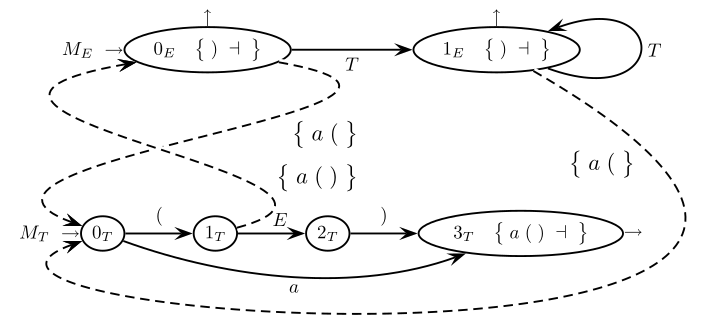
\includegraphics[width = \textwidth]{./images/PCFG.png}
					\end{figure}
			 
			\subsubsection{ELL test}
				Given the PCFG, we can easily check if an automata is ELL by exploiting a corollary of the ELL condition itself, which states that a machine network 
				satisfies ELL iff for each state, all the outgoing arcs' guide sets are disjoint. The double implication means that building the PCFG and checking 
				the disjointness of the guide sets proves if a machine network satisfies ELL or not.

				\emph{\textbf{This means we can avoid building the pilot automaton to check for ELL property}}
				
			\subsubsection{Possible implementation techniques}
				This short paragraph explains how to implement a predictive parser (but not why, tho) by means of two of the most common techniques.
				\begin{itemize}
					\item Recursive procedures: every submachine is encoded as a single procedure that scans the input tape char by char and that analyzes the input 
					token as the automaton would: guide sets and arc labels are used to build the patterns to match the current character against. Termination of a 
					subprocedure: acceptance; else an error is thrown. To recognize a nonterminal the associated procedure is called. (A lot of talking for an 
					implementation technique that's really simple in practice: just modularize the code according to the machines in the network).
					\item Explicit stack: this method does not take advantage of the recursiveness to memorize the state of the application, instead it saves it on 
					the stack directly. The parser can perform 4 different moves (here with "replace q with r" is intended pop q push r):
						\begin{enumerate}
							\item scan: if the shift arc q $\rightarrow$ r exist, then q is replaced with r.
							\item call: move performed when a submachine is invoked. Pop of the current state, push of the first state after call (so if 
							$q \xrightarrow{B} r$ replace q with r and push $0_B$), push of the first state of the called machine.
							\item return: the next character is in the prospect set of the current state, which is final: pop.
							\item recognition: if we are in the final state of the axiom machine and the current character is $\dashv$, recgnize and halt. Otherwise, 
							error and halt.
						\end{enumerate}
				\end{itemize}
				
			\subsubsection{Lookahead lenghtening}
				Often it's sufficient to increase the lenght of the lookahed (to more than one token) to render a top down parser deterministic fom a non-ELL grammar. 
				In this course, the only method is a "eagle eye" one where you spot the perfect lenght just looking at the PCFG and choosing which minimum lookahed 
				set grants determinism, basing yourself on pure parser instinct.
				
		\subsection{Earley algorithm}
			The Earley algorithm is a method to recognize strings from a grammar even if this is ambiguous. The pseudocode approach both the book and the slides take 
			is very counterintuitive, in my opinion. So, I will try just to explain \emph{how practically} a Earley recognizers is built and used. Keep in mind that 
			this procedure should build \emph{a software}.

			First, initialize the vector of candidates to E = \{ $\langle 0_s, 0 \rangle$ \} that represent the initial state and the first value

			Then, with $n$ taken as the lenght of the string to recognize, we initialize all the elements of E[1..n] to the empty set.

			We complete the first element E[0]. Completing an element (applying the \emph{completion} operation to it) means computing the closure of the state (and 
			adding to the E[i] set of candidates the closure's states) and calculating also all the states that are reachable through a nonterminal shift (watch out: 
			with nonterminal shift we are referring to the operation of "arriving on E[i] with a nonterminal shift", not leaving this state), adding them also to the 
			state.

			We then compute, for every token in the string, the \emph{terminalshift} for every element in the vector (terminalshift means nonterminalshift with 
			terminal symbols. For every candidate in previous state that can terminalshift to a candidate in the current state add that transiction [represented as 
			the candidate $state, index - 1$] to this vector element) to build the shifting operation, then we complete it.

			This algorithm is similar to the method to build a pilot automaton, but instead of lookahed sets just the position in the vector of the caller state is 
			memorized. The string is accepted if the last element of the vector is of type $\langle finalstate, 0 \rangle$: this means that the condition is 
			accepting (finalstate) and the whole string is accepted (0).
			
			These example and notation should clear all remaining doubts:
			\begin{figure}[H]
				\centering
				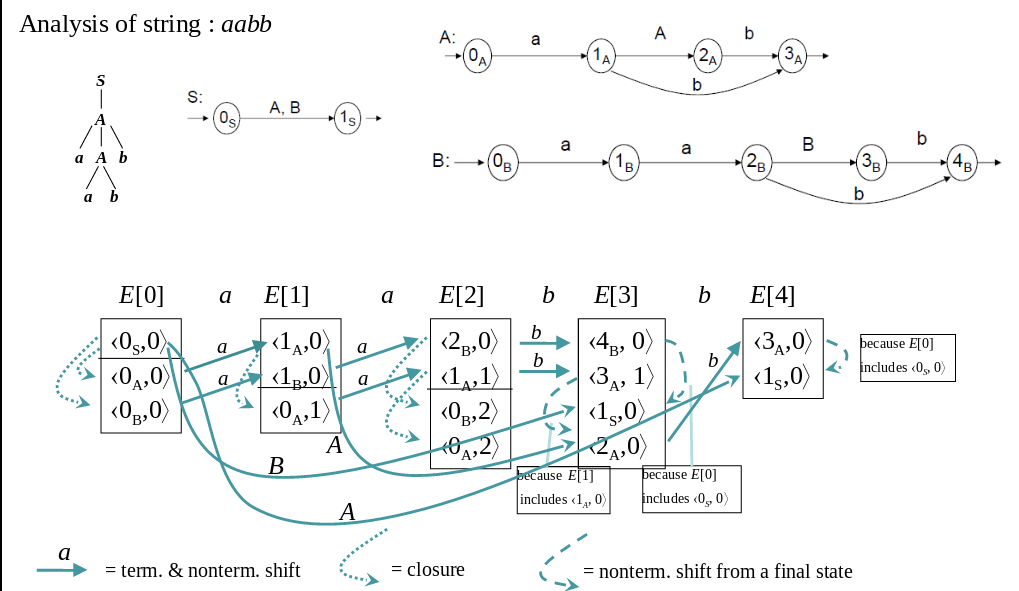
\includegraphics[width = \textwidth]{./images/exEarley.png}
			\end{figure}
	\chapter{Translation and Static Analysis}
	What is translation (mathematically speaking)? Let $\Sigma$ and $\Delta$ be two alphabets (\emph{source} and \emph{target} respectively); a translation is a 
	correspondence between source and target strings, that is formalized by binary realtion between the source and target universal languages (that is $\Sigma^\ast$ 
	and $\Delta^\ast$). Formally, a translation is a subset of $\Sigma^\ast \times \Delta^\ast$. So, it can be also seen as a function, and inherits all the 
	function's peculiar properties (like surjectivity, injectivity and all the terminology that concerns dominion, image and inverses).
	
	\section{Purely Syntactic Translation}
		\subsection{Translation Grammars}
			When the source language is generated by a grammar, one of the most natural translation is to map each subtree to a target subtree. This is done by 
			building a \emph{translation grammar} that have the same number of rules of the source language grammar and differs only in the terminal symbols in 
			the right part of the rules. The nonterminals symbols are \emph{the same and in the same order}.

			A typical example of translation grammars come from bynary functions notation, when translatin the classic infix notation ($A \times B$) into a 
			pre/postfix polish notation, like $\times A B$ that's way more concise and understandable, being less prone to error caused by operator's precedence.

			We have so a grammar for the infix notation expression, and one that describes the target language, a prefix polish notation:
			\begin{equation}
				\begin{cases}
					E \rightarrow E + E \\
					E \rightarrow E * E \\
					E \rightarrow ( E ) \\
					E \rightarrow i
				\end{cases} 
				\begin{cases}
					E \rightarrow \text{add } E \text{ } E \\
					E \rightarrow \text{mult } E \text{ } E \\
					E \rightarrow E  \\
					E \rightarrow i
				\end{cases}
			\end{equation}
			So we build our translation grammar this way:
			\begin{equation}
				\begin{cases}
					E \rightarrow \frac{\epsilon}{add} E \frac{+}{\epsilon} E \\
					E \rightarrow \frac{\epsilon}{mult} E \frac{*}{\epsilon} E \\
					E \rightarrow \frac{(}{\epsilon} E \frac{)}{\epsilon} \\
					E \rightarrow \frac{i}{i} \\
				\end{cases}
			\end{equation}
			
			\subsubsection{Ambiguity}
				If the source grammar is ambiguous then the translation scheme is ambiguous: if a sentence can be generated bby more than one syntax trees, 
				obviously the translator should take care of this multi-valued rules. Ambiguity in the translation grammar can also derive by duplicated rules, 
				that can be mapped to different values: in this case, both the source and target grammar are unambiguous, but multiple translation rules correspond 
				to the same source rule, rendering the translation grammar multi-valued $\Rightarrow$ ambiguous.

				Summing up these two concepts, a translation grammar $ G_\theta = \{ G_1 , G_2\}$ is unambiguous (single-valued) if 
				\begin{enumerate}
					\item $G_1$ is unambiguous;
					\item No two rules of target grammar $G_2$ map on the same $G_1$ rule.
				\end{enumerate}
		
		\subsection{Pushdown Transducer}
			We have defined a translation between grammars, now we have to define a machine that performs it. Such machine is a \emph{pushdown transducer}, so a 
			pushdown automaton with output capabilities. It has the same definition of a PDA, enriched with the output (target) alphabet, and with a different 
			transiction function: in fact, this should now take into account also the output of the machine, not only the state transitions.

			\emph{A translation relation is defined by a translation grammar iff it is computed by a nondeterministic pushdown transducer}. This property ensure 
			the equivalence of the two methods, and also grants the possibility of defining a machine starting from the grammar as in traditional parsing. 
			
			\subsubsection{Single state nondeterministic transducer}
				Theoretically speaking, the simplest extension from a parser to a transducer is built directly associating to the grammar rules some move, this time 
				adding the write operation. We obtain a nondeterministic single state transducer, with not the minimal practical value.
			
			\subsubsection{ELL grammars translation}
				ELL parsers can be implemented by recursive function calls (classic top down approach), as explained in (21.4.3). Extending the recursive calls 
				parsers with write functions just after the submodule call is enough to render the parser a transducer. Simple as that. Remember that ELL parsers 
				rely on a stronger assumption then ELR, so they're less complex and easier to extend; they're also applicable to a reduced number of cases.
			
			\subsubsection{ELR grammars translation}
				ELR parsers are not easily extended as their ELL brothers. In fact, just adding the output action after a shift operation could lead to contradictory 
				writes, becaouse of the inherent nondeterminism of the bottom up approach to parsing. Instead, the reduce operation grants the recognition of a 
				single grammar rule, and (due to the total mapping of the source to the target rules) one target rule can be identified and selected for output.

				This is easier said than done: a reduction could take place before another that may need to write a characte \emph{before} the current one; to avoid 
				this kind of phenomena, the translation grammar must be in \textbf{postfix normal form}: a translation grammar is in postfix normal form when all its 
				rules are of the kind
				\begin{equation}
					A \rightarrow \Sigma^\ast \delta^\ast
				\end{equation} 
				so they produce the output strings \emph{only} at the end of the rules as a suffix of the production, and not in the middle of it.

				To convert a grammar in the postfix normal for it's enough to replace all the terminals in the translation that violates the postfix form with new 
				nonterminals that simply produces the substitued character (this change should be reflected in the target grammar also). A translation grammar in 
				the postfix normal form ensures that, when implemented via an automaton, the output operations take place only at reduction time. This trnsformation 
				makes sure that the construction of a pilot automaton for a \emph{transducer} is identical to the one for a \emph{parser} with just the write 
				operation added to the m-states that have a final state in them.

				In some particular cases (that are indeed very rare, according to the literature) normalizing a grammar can introduce shift reduce conflicts due to 
				the introduction of initial - final states in the automaton.
			
			\subsubsection{Regular Translation}
				\paragraph{Regular Languages Translation}
					As regular expression are a proper subset of CF grammars, they have a special family of transducers. Consider this translation grammar:
					\begin{equation}
						G_\tau = 
						\begin{cases}
							A_0 \rightarrow \frac{a}{c}A_1 \,\vert\, \frac{a}{c} \,\vert\, \frac{a}{b}A_3 \,\vert\, \epsilon \\
							A_1 \rightarrow \frac{a}{c}A_2 \,\vert\, \epsilon \\
							A_2 \rightarrow \frac{a}{c}A_1 \\
							A_3 \rightarrow \frac{a}{b}A_4 \\
							A_4 \rightarrow \frac{a}{b}A_3 \,\vert\, \epsilon 
						\end{cases}
					\end{equation}
					\textbf{Things to be noted}:
					\begin{enumerate}
						\item the grammar translates string of "a" in strings of "b" when the number of "a" is even
						\item the grammar translates string of "a" in strings of "c" when the number of "a" is odd
						\item to "count" the number of letters, the grammar constructs two loops ($A_0 \rightarrow A_1 \rightarrow A_2 \rightarrow A_1$ and 
						$A_0 \rightarrow A_3 \rightarrow A_4 \rightarrow A_3$) to either create an odd number of letters or an even one. This can be noted observing 
						which rules contains the empty string in the loop
						\item the grammar is right linear (so? it's equivalent to a regular expression)
						\item the grammar is in prefix normal form (does this have some relevance now? no)
					\end{enumerate}
					As well as a right linear grammar can easily be converted in a regular expression, we can derive a \emph{regular transducer} that translates the 
					language of this translation grammar. It's pretty straightforward:
					\begin{equation}
						e_\tau = \left(\frac{a^2}{b^2} \right)^\ast \,\cup\, \frac{a}{c} \left(\frac{a^2}{c^2} \right)^\ast
					\end{equation}
					
				\paragraph{Two Input Automaton}
					Starting from the defined "regular translator" in the previous paragraph, we can see that the combination of terminals of the source and 
					target expressions can be seen as a terminal alphabet itself (it will be a terminal alphabet built on the cartesian product of two alphabets, 
					but the idea is there). So, with the regular expression $\leftrightarrow$ FSA equivalence in mind, we can define a FSA that recognize (validates) 
					the translations of the source expressions. This machine will ha ve \emph{two} input tapes, one for the source and one for the target terminals, 
					and will recognize the input when it's a valis translation. The only thing that's odd about 2I-FSA is the way empty strings are managed: if the 
					transiction function accepts a empty string as input character \emph{on one of the two tapes}, the machine could still be blocked by the reading 
					on the other one.

					As an example we produce the 2I-FSA that recognizes the translation of the above regular translation.
					\begin{figure}[H]
						\centering
						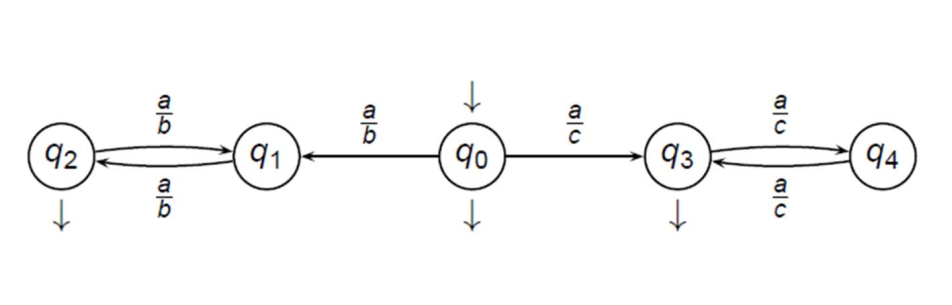
\includegraphics[width = \textwidth]{./images/2IFSA.png}
						\caption{To be noted: this automaton is deterministic, because the two moves exiting from $q_0$ have different labels}
					\end{figure}
					
				\paragraph{Finite Transducer}
					We want an automaton that formalizes the translation (REMINDER: A 2I-FSA DOES NOT TRANSLATE, BUT VALIDATES A TRANSLATION) so that starting from a 
					string on an input tape prints the translated string on an output one. The schema is very simple:
					\begin{figure}[H]
						\centering
						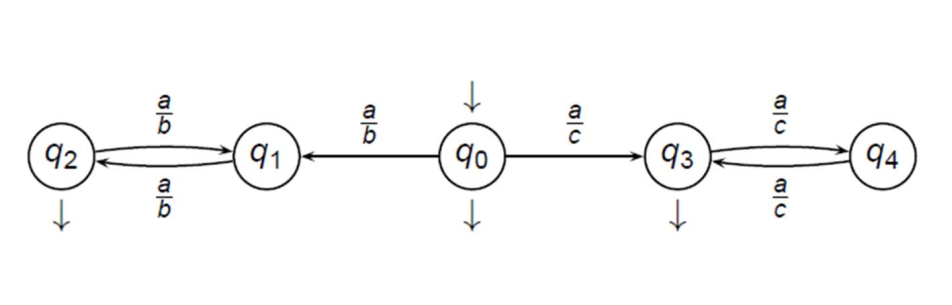
\includegraphics[width = \textwidth]{./images/2IFSA.png}
					\end{figure}
					Is it familiar? It's the \emph{same} formalization as the 2I-FSA that validates the translation, but this time the labels have a 
					\textbf{totally different meaning}: the bottom character represents the one printed on the output tape. So, this time the automaton is 
					nondeterministic, because of the two arcs exiting from $q_0$ have the same input character; only one of the two will make the automaton 
					finish in an acceptance state; this also means that \emph{no output can be produced until a final state is reached}.
					
				\paragraph{Sequential Transducer}
					Ok, now we want a machine that translates input \emph{real time}, so while scanning the input tape (to overcome the limitation of finite 
					transducers that must reach a final state to print). The sequential transducer model differs from the aforementioned ones in the theoretical 
					representation (it makes use of three functions: a transition one, an output one, and a \emph{final} one) but not in the graphical rep. The 
					core idea is very similar to the finite transducer but the output characters are \emph{actually} printed as output. This model needs an 
					additional function that computes the "string terminator": the so called final function, in fact, just appends to the translated string a 
					marker that signals the end of the translation, and the final state reached by the computation.

					This may seem overly complicated, let's use an example to clarify: a sequential transducer that eliminates all the leading zeroes from a 
					string. The input string are built on a alphabet composed of three characters, \{ $0, 1, \sqcup$ \} where $\sqcup$ represents the separator 
					between values. If a string is composed solely by zeroes, a single zero is outputted.
					I'll skip the definition of the regular translation expression for this automaton, to present directly the machine:
					\begin{figure}[H]
						\centering
						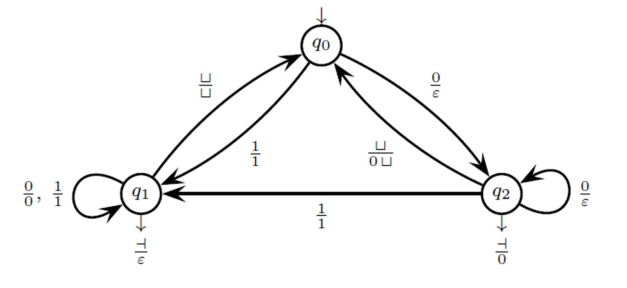
\includegraphics[width = \textwidth]{./images/SeqTrans.png}
					\end{figure}
					The above machine can be explained section by section:
					\begin{enumerate}
						\item state $q_2$ carries out the meaningless zeroes. She outputs nothing, never, exception made for when the terminator is read, when a 
						single zero is written. 
						\item state $q_1$ takes care of the meaningful part of the string. It's reachable through a scan of the character "1", that signals the start 
						of the meaningful part of the string; its only task is to traduce the string as is.
						\item $q_0$ interpret blank spaces. 
					\end{enumerate}
					
	\section{Syntax Directed Translation}
	
		The compilation process cannot be performed only through syntactic methods. A \emph{meaning} must be assigned to sentences, and (while this can be 
		accomplished in a formal way) the only "structured reading and translation" of a sentence is not enough to do so. Syntax directed translators starts from the 
		syntax trees of a grammar and enrich them with semantic attributes. 
		
		\subsection{Attribute Grammars}
			Attribute grammars have the same computing expressiveness of Turing machines (they are very powerful). They are the third step of computations during a 
			compilation procedure: they are preceded only by lexical and syntactic analysis. The purpose of attribute grammars is to help design the 
			\emph{decorated syntax tree} that enriches the normal s.t. with a semantic value.

			Let's run an example:
			
			\paragraph{Meaningful example}
				We'll build an attribute grammar for the language $L = \{0, 1\} \,\bullet\, \{0, 1\}$ that represents decimal numbers in a fixed point fashion. The 
				grammar that generates it is
				\begin{equation}
					G_L = 
					\begin{cases}
						N \rightarrow D \bullet D \\
						D \rightarrow D \, B \, \vert \, B \\
						B \rightarrow 0 \, \vert \, 1
					\end{cases}
				\end{equation}
				Where N is the axiom, D is the string, B is the single bit. The goal of our attribute grammar is to compute the decimal value of each part of the 
				number, assigning the real weight to the single bits. To do so, we need to keep track of two fundamentals attributes:
				\begin{enumerate}
					\item The value of the numeric parts of the string: the N, D and B nonterminals have all this attribute, because they are all \emph{semantically} 
					numbers;
					\item Their position in the string; an easier way to compute so is to keep track of the string lenght. Only nonterminal D needs this attribute. 
					N does not need it because it's just a concatenation of two values. 
				\end{enumerate}
				So, now we have a grammar and a set of attributes with a semantic value that must be linked to certain nonterminals. To do so, we can define 
				functions (associated to every production) that computes the value of the nonterminal of the reduction. In this case:
				\begin{equation}
					G_{L_ext} = 
					\begin{cases}
						N \rightarrow D \bullet D \text{ sum of the right with the left part: } v_0 = v_1\,+\,v_2\times 2^{-l_2} \\
						D \rightarrow D \, B \, \vert \, B \text{ also consider the length increase: } 
							\begin{cases}
								\begin{cases}
									v_0 = 2 \,\times\, v_1\,+\,v_2 \\
									l_0 = l_1 + 1
								\end{cases}\\
								\begin{cases}
									v_0 = v_1 \\
									l_0 = 1
								\end{cases}
							\end{cases}\\
						B \rightarrow 0 \, \vert \, 1 \text{ just assign the final value to the nonterminal: } 
							\begin{cases}
								v_0 = 0\\
								v_0 = 1
							\end{cases}
					\end{cases}
				\end{equation}
				A detailed explanation of what $l_0, l_1, v_0, v_1 \text{ and } v_2$ are is needed: the letter is the attribute we're referencing 
				($l = \text{ lenght and } v = \text{ numeric value}$) and the pedix symbolizes the \emph{cardinal position of the nonterminal we are considering}: 
				this means that all the attributes that have the zero pedix will be the results of the computation, because they are the attributes of the left part 
				of the grammar rule. Vice versa, $v_2$ represents the numeric value of the \emph{third} nonterminal in the rule.

				The computation evolves around the tree in this way:
				\begin{figure}[H]
					\centering
					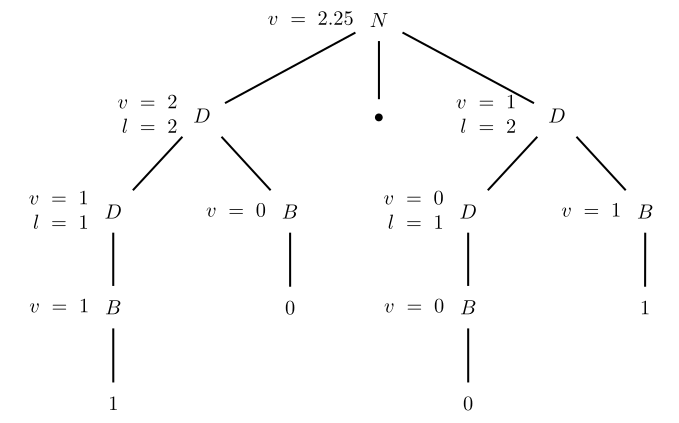
\includegraphics[width = \textwidth]{./images/decoratedTree.png}
				\end{figure}
				
			\subsubsection{Left and Right Attributes}
				The definition of left and right attributes is as tricky as fundamental for the comprehension of attribute grammars. Let's try to figure it out:
				\paragraph{Left attributes}
					We want to generate a value from a production, what did we do in the previous example? We computed the value for the right part recursively till a 
					fixed point (the production that has associated a function that produces a costant, such as $l_0 \,=\, 0$). In this case, $l_0$ is a left 
					attribute, because it's associated with a left part of the rule. Left attributes are also called "synthetized" because they usually represents the 
					result of the computation.
				\paragraph{Right attributes}
					We say that an attribute is "right" or "inherited" if it's associated to a right part of a rule, so the functions that calculate it has as output 
					not a value that goes in the left part of the rule, but stays in the right part.
				\\\\Still nebolous definitions, and no practical value. Let's make an example, \emph{read it carefully}:

				we have as input a string of words, separated by blank spaces (we will represent them with $\dashv$). We want to arrange the text into rows of fixed 
				length $W$ and compute for each word the column of its last character. We assume no words have length that's greater than $W$. 
				\begin{equation}
					G = 
					\begin{cases}
						S \rightarrow T \\
						T \rightarrow T \dashv T \\
						T \rightarrow V \\
						V \rightarrow cV \,\vert\, c
					\end{cases}
				\end{equation}
				The "c" terminal respresents any character. Which attributes are needed?
				\begin{itemize}
					\item \emph{last} stores the column of the last letter
					\item \emph{length} stores the length of the word
					\item \emph{prec} is the column of the last character of the previous word
				\end{itemize}
				These three attributes are all we need to describe the set of words, element by element. The idea is to compute the last character of each word as: 
				$last = prec + 1 + lenght$. It's pretty straightforward spotting the only right attribute: \emph{prec}. In fact, it's extracted from the left part of 
				the rule. Let's define all the functions associated to the rules.
				\begin{center}
					\begin{tabular}{| m{3cm} || m{3cm} | m{3cm} | }
						Rule & Left attributes & Right attributes \\
						\hline
						$S \rightarrow T$ & & $prec_1 = -1$\\
						\hline
						$T \rightarrow T \dashv T$ & $last_0 = last_2$ & $prec_1 = prec_0\,\,\,prec_2 = last_1$ \\
						\hline
						$T \rightarrow V $ & $last_0 = (prec_0 + lenght_1 + 1 > W) ? lenght_1 : (prec_0 + lenght_1 + 1)$ &\\
						\hline
						$V \rightarrow cV$ & $lenght_0 = 1 + lenght_1$ & \\
						\hline
						$V \rightarrow c$ & $lenght_0 = 1$ &  
					\end{tabular}
				\end{center}
				Let's describe what's each function do:
				\begin{itemize}
					\item Left attributes:
					\begin{itemize}
						\item $last_0 = last_2$ stands for "the last element of two words is the last element of the last word".
						\item $last_0 = (prec_0 + lenght_1 + 1 > W) \,?\, lenght_1 \,:\, (prec_0 + lenght_1 + 1)$ this function (expressed as a inline if instruction) 
						verifies if we've reached the end of the line, composed of $W$ coloumns. If we are (the condition is true) we've reached the first word of the 
						next line, so the lasta character of this word will be on the last coloumn. Otherwise, it will be taken into account also the lenght of the 
						preceding word.
						\item  $lenght_0 = 1 + lenght_1$ and $lenght_0 = 1$ are classical recursive calls to form the words lenght.
					\end{itemize}
					\item Right attributes:
						\begin{itemize}
							\item $prec_1 = -1$ initializes the first word's predecessor.
							\item $prec_1 = prec_0$ and $prec_2 = last_1$ sets the value of the predecessor for each word. Note how the information, in this case, 
							flows downward to the leaves: to be set are the values of attributes that only later in the execution will be utilized. In this case: 
							we're setting the predecessor of each word: predecessor of the first = last one's predecessor and second one's predecessor = last 
							character of the first.
						\end{itemize}
				\end{itemize}
				The final decorated tree is:
				\begin{figure}[H]
					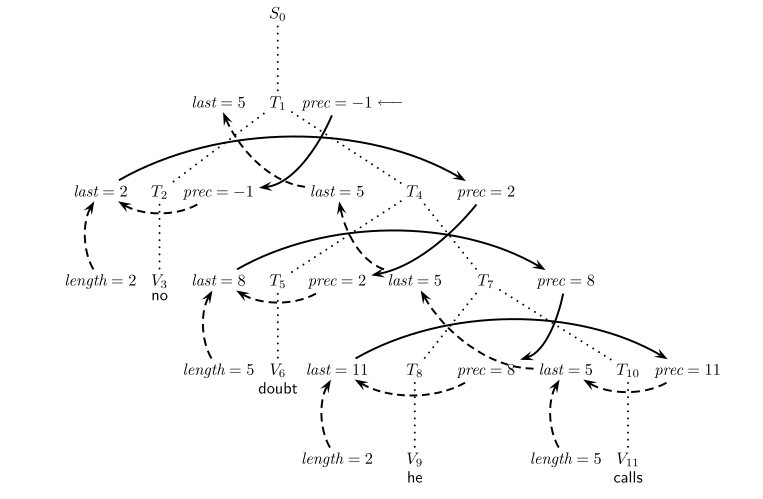
\includegraphics[width = \textwidth]{./images/decTree.png}
				\end{figure}
				Let's formalize all this reasoning:
			
			\subsubsection{Formal Definition of an Attribute Grammar}
				An attribute grammar is composed of:
				\begin{enumerate}
					\item A context-free grammar $G = \langle V, \epsilon, P, S \rangle$ with her set of terminals, nonterminals and the axiom. It is convenient to 
					NOT have the axiom in the right part of the rules
					\item A set of semantic attributes, associated with terminals and nonterminals. This set is separated in left attributes and right attributes: 
					\emph{the two sets are disjoint. No right attribute can be left attribute in another production and vice versa}. The set of attributes of 
					nonterminal D is also referred to as $attr(D)$
					\item A set of semantic functions, each associated with a grammar rule. The grammar rule associated with each function is called the support of 
					that function. In general, several functions can have the same support, and the set of functions supported by production p is $fun(p)$. Semantic 
					functions are formally defined as:
						\begin{equation}
							\begin{cases}
								\text{the support: } p = D_0 \rightarrow D_1 D_2 ... D_r\\
								\text{the function: } \sigma_k = f(attr(\{D_0, D_1, ..., D_r\}) \backslash \{\sigma_k\})\\
								r \geq 0\\
								0 \leq k \leq r
							\end{cases}
						\end{equation}
					\item All the semantic functions must respect:
						\begin{enumerate}
							\item For each left attribute of a left nonterminal of a production there is \emph{exactly one} function that defines it
							\item For each production, no functions defines \emph{right attributes for the left side nonterminals}
							\item For each production, no functions defines \emph{left attribute for the right side nonterminals}
							\item For each right attribute of a right nonterminal of a production there is \emph{exactly one} function that defines it
						\end{enumerate}
						These four rules better regulates the "attributes placements and initialization": in fact, they states that all the left-hand side 
						nonterminals can have only left attributes and also that such attributes must be uniquely defined; also they states that for all 
						right-hand side nonterminals only left attributes are possibly defined and \emph{also} they are uniquely defined. The other attributes are 
						called \emph{external attributes}, because they're not comupted in the function.
				\end{enumerate}
				
				\paragraph{Dependence Graph}
					The graph showed in 23.1.1 is a complete dependence graph obtained by "summing" all the graphs of its subtrees. The single dependence graph can be 
					referred to semantic functions, or to productions (so \emph{to all} the semantic functions that have that rule as support). The decorated syntax 
					tree, ultimately, is the complete dependence graph of all the productions.

					How to build a decorated tree, even though it's far from Christmas: just link the arguments of the function to the attribute that function 
					initializes. So, if the function is $attr_0 = f(\{attr_1, attr_2\})$ in the decorated graph we will have something like 
					$attr_1 \rightarrow attr_0 \text{ and } attr_2 \rightarrow attr_0$.
			
			\subsubsection{Grammar Validation}
				Given an attribute grammar defined as before, if the dependence graph of the tree is acyclic, there's a set of attribute values consistent with the 
				dependences. A grammar is loop free id \emph{every dep graph of every tree} is acyclic. How to test if a grammar is acyclic? Given the infite number 
				of syntax trees, computing all of them to check for cycles is not viable. Instead, it's enough to ensure certain properties, that are sufficient to 
				guarantee the desired condition of acyclicity.
				
				\paragraph{One Sweep Grammar}
					"One sweep" is a property that ensures that a grammar can be evaluated with a depth first visit. What does this mean? It means that 
					\emph{it's possible to perform attribute evaluation during a depth first visit}. Why should this be checked? Because the depth first visit 
					operates this way:
					\begin{enumerate}
						\item before entering a subtree compute all right attributes of the root of that subtree
						\item when "emerging" from a visit of a subtree, compute all the left attributes of the root of that subtree
					\end{enumerate} 
					Both these two operations can get stuck in the evaluation of certain attributes, because of the possible functional dependences among attributes. 
					A one sweep grammar is ensured to be free of such problems.

					So how to check for "onesweepness"? We shall recall the definition of the $dep$ set, and introduce the \emph{sibling graph}:
					\begin{enumerate}
						\item The nodes are the right symbols of the productions $\{D_1\,...\,D_r\}$.
						\item Arcs $D_i \,\rightarrow\, D_j$ are drawn between nodes that have an attribute dependency like 
						$\sigma_{D_i} \,\rightarrow\, \theta_{D_j}$. The nodes in the siblings graph \textbf{are not} the ones of the dependence graph of the 
						production. 
					\end{enumerate}
					Let's generate a sibling graph for a dummy rule, $D\rightarrow A\,B\,C$ that has the dependency graph as below:
					\begin{figure}[H]
						\centering
						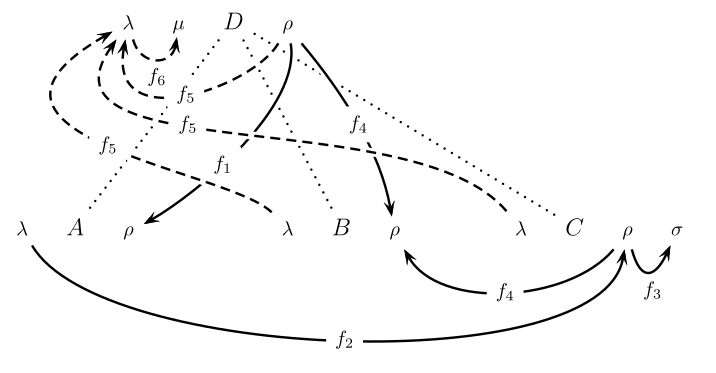
\includegraphics[width = \textwidth]{./images/dummyRule.png}
					\end{figure}
					The resulting sibling graph is:
					\begin{figure}[H]
						\centering
						
\includegraphics[width = \textwidth]{./images/sibling.png}
					\end{figure}
					For a grammar to have the one sweep property it must hold, for all the productions:
					\begin{enumerate}
						\item $dep_p$ contains no circuits;
						\item $dep_p$ contains no path that goes from a left attribute to a right attribute of the same node;
						\item $dep_p$ contains no arc from the left attribute of a father to a right attribute of a children;
						\item $sibl_p$ contains no circuits. 
					\end{enumerate}
			
			\subsubsection{Validation of a Grammar through a One Sweep Evaluator}
				The algorithm we described before to visit a tree depth first can be formalized to generate a one sweep evaluator, a machine that carries out all the 
				computation of an attribute grammar. REMEMBER: the evaluator built this way \emph{relies} on the assumption that the grammar is one sweep.

				A semantic procedure is written for each \emph{nonterminal}: this procedure has as arguments the subtree generated by that nonterminal and his right 
				attributes. The procedure must, for every support rule $p: D_0 \,\rightarrow\, D_1\,...\,D_n$ with $n \geq 0$
				\begin{enumerate}
					\item Choose the TOS (Topological Order for Siblings) for $\{D_1\,...\,D_n\}$ wrt the sibling graph for that nonterminal
					\item Choose the TOR (Topological Order for Right attributes) for all the right attributes of all symbols $\{D_1\,...\,D_n\}$ wrt the dependence 
					graph of that symbol
					\item Choose the TOL (you guess. Hint: opposite of right...)
				\end{enumerate}
				These three \st{demigods} orders prescribe \emph{how to arrange the instructions} in the procedure body. To explain that, we'll make as example the 
				procedure that is generated by the rule in the previous example, $D \,\rightarrow\, A\,B\,C$, with the dep graph as shown before. This grammar is 
				easily proven one sweep (the sibling graph has no cycles and no cycles or cross dependecies are seen in the dep graph).

				The procedure starts of choosing a TOS: due to the sibling graph's arcs, the order choosen is $\{A,\,C,\,B\}$.

				Then she chosses the TOR, taking into consideration the dependencies shown in $dep$: $\rho\,\rightarrow\,\sigma$ is the one.

				Last but not least TOL: again, watching the dependencies, we have $\lambda\,\rightarrow\,\mu$.

				Once these three orders are identified, the procedure can be written: I'll try to give an abstract explanation of \emph{how} the three orders are 
				used (because I hate pseudocode) then I'll add a pseudocode example.

				Subtrees are computed in TOS order, and for each subtree the "computational pattern" is
				\begin{enumerate}
					\item compute right attributes in TOR order using the functions highlighted in $dep$
					\item call the subprocedure of that symbol passing as argument also the attribute to popolate
					\item compute left attributes with the assigned functions in TOL order
				\end{enumerate}
				
				So in this case, the procedure becomes:\\
				def D ( in: root, $\rho_D$, out: $\lambda_D$, $\mu_D$):\\
			    $\rho_A = f_1(\rho_D)$\\
			    $A(root_A, \rho_A; \lambda_A)$\\\\
				$\rho_C = f_2(\rho_A)$\\
				$\sigma_C = f_3(\rho_C)$\\
				$C(root_C, \rho_C, \sigma_C; \lambda_C)$\\\\
				$\rho_B = f_4(\rho_C, \rho_D)$\\
				$B(root_B, \rho_B; \lambda_B)$\\\\
				$\lambda_D = f_5(\lambda_B, \lambda_C, \rho_D)$\\
				$\mu_D = f_6(\lambda_D)$\\
	
	\subsection{Combined Syntax and Semantic Analysis}
		In some cases syntax analysis and attribute evaluation (semantic analysis) can be performed at the same time. For each class of languages we've seen, a 
		different approach can be developed.
		
		\subsubsection{Regular Laguages - Lexical Analysis with Attribute Evaluation}
			If the language is regular, then the \emph{scanner} or \emph{lexxer} 's task is to identify and isolate \emph{lexemes}, the minimal tokens of a language 
			that can be given a semantic weight. The scanner can also give attributes to these tokens, and compute them.
		
		\subsubsection{LL Languages - Attribute Recursive Descent Translator}
			If the syntax is suitable for top down parsing (is LL) and the grammar is one-sweep, it's necessary to add just another hypothesys to make sure that the 
			parsing and the semantic analysis can procede step by step together. The condition to be satisfied is the L condition, that states:\\
			a grammar satisfies the L(eft to right) condition if
			\begin{itemize}
				\item It's one-sweep
				\item The sibling graph (of every support) contains \textbf{no arc} so that $D_i \,\rightarrow\, D_j$ with $j > i \geq 1$ (so no 
				\emph{backward dependency})
			\end{itemize}
			If the syntax is LL and the L condition is satisfied (what is wrong with the letter L I would like to know) then a 
			\emph{attribute recursive descent translator} can be built \footnote{I know, it sounds like a General Zod weapon, doesn't it?}.

    \section{Static Analysis}
            \subsection{Compilation of a Program}
                Compilers are composed of two part: a front end compiler (that translates the actual source code into a "lower level code". This is made possible by 
				a scanner + parser pipeline) and a back end compiler (that takes the lower level code and generates the executable). After the front end compiler has 
				generated the intermediate representation of the program, this goes through three additional phases:
                \begin{enumerate}
                    \item \textbf{Verification} correctness check
                    \item \textbf{Optimization} target specific improvements to enhance performance
                    \item \textbf{Scheduling} modification of the produced code to fully use the pipelines/parallel capabilities of the machine
                \end{enumerate}
                
                \subsubsection{Control Flow Graph}
                    To analyze the program in these three further phases, a schematic representation of the program itself is needed. This representation is usually 
					a control flow graph, that stands for an automaton. Needless to say, this automaton is the same \emph{formal structure} of the ones used to 
					interpret the source code, but has a \emph{totally diffferent meaning}: this automaton in fact describes the program itself and the use it makes 
					of the variables.
                    
                    \paragraph{How to Build a CFG}
                        CFGs are simple def-use graphs. They do \emph{not} represents the logic unfolding of the program, but just the usage of the memory. The 
						following abstractions are utilized:
                        \begin{itemize}
                            \item All the conditional statements are not represented
                            \item "Instruction B follows instruction A" is drawed out as the classic arc
                            \item All operations are reduced to two sets: \emph{def} and \emph{use}. These two sets represents the group of variable to which a value 
							is assigned and the group of variables which value is read
                        \end{itemize}
                        So far, we've defined an automaton with some sets. But which strings does this automaton recognizes? A string recognized by an automaton 
						described by means of a CFG is a possible \emph{execution trace} of the program, or the execution path that traverse a valid sequence of 
						instructions. In these pages, we will consider onyl \emph{intraprocedural} static analysis, that is performed \emph{in isolation} on every 
						procedure.
                    
                    \paragraph{Conservative Approximation}
                        The choice to ignore the unreachable path enables the analyzer to reach unreachable segments of code. This could lead to pessimistic outcomes 
						(like a program is deemed invalid or with errors, but these errors are all located in an unreachable segment). This condition is called 
						conservative approximation because "pessimistic conclusions" are far preferrable rather than "optimistic conclusions": the latter can lead 
						to assign a smaller-than-needed amount of resources, while the former never misses an error.
                
                \subsubsection{Liveness Intervals Analysis}
                    Variable liveness analysis is used to discover definition errors or clashes or unreferenced accesses. A variable \emph{a} is said to be "live" on 
					the \emph{exit} of a node \emph{p} if there exists a path between \emph{p} and another node \emph{q} so that \emph{a} does not appear in 
					\emph{any} def sets of the traversed nodes, but it appears in the use set of \emph{q}.

                    This definition is usually referred to as "live-out", because it takes in consideration the exiting arcs from a node. A specular formulation 
					("live-in") can be given. Example of usage: if a variable is defined in a certain node, but it's not live-out of that node, the assignement can 
					be deleted without altering the program behaviour.
                    
                    \paragraph{Computing Liveness Intervals - Data Flow Equations}
                        The scary name of "data flow equations" is given to a rather simple approach to the problem of calculating all the $live_in$ and $live_out$ 
						sets for each node of the control flow graph. The procedure is inherently recursive and starts from the final nodes. It unfolds this way:
                        \begin{equation}
                            \forall p \in CFG \,\vert\, p \in Finals \Rightarrow live_{out}(p) = \emptyset
                        \end{equation}
                        So (quite logically) if a node is final his live out variable set is empty. Next equation (that represents the "recursive call") makes use of 
						the $succ$ set, representing all the \emph{immediately reachable nodes} from a given one.
                        \begin{equation}
                            \forall p \in CFG \,\vert\, live_{out}(p) = \bigcup\limits_{\forall q \in succ(p)} live_{in}(q) 
                        \end{equation}
                        \begin{equation}
                            \forall p \in CFG \,\vert\, live_{in}(p) = use(p) \cup (live_{out}(p) \backslash def(p))
                        \end{equation}
                        The sketched procedure is quite simple: starting from the last nodes, the CFG is traversed backwards adding time to time to each node his 
						$live_{in}$ and $live_{out}$ sets. For every node that's not final, the $live_{out}$ set si composed of all the variables in the $live_{in}$ 
						sets of his successors. The $live_{in}$ set instead is composed of all the used variables in that node plus the $live_{out}$ set purged from 
						the redefined variables (doubts? check the "liveness" condition definition for a variable).
                        
                    \paragraph{Applications}
                        Liveness analysis is performed during
                        \begin{itemize}
                            \item Memory allocation: if two variables \emph{interfere} with each other (so they're both present in the live-in set of a node on the 
							CFG) they must be both present in memory when such point is reached. If this does not happens, a cell of memory can be used to store both 
							the variables, at different times. This is a useful performance enhancement. 
                            \item Useless definitions: as exemplified before, a definistion is useless if the defined variable is not in the live-out set of the 
							instruction defining it. A condition like this emerges from the liveness analysis, and can lead to heavy code-cleaning. 
                        \end{itemize}
                
                \subsubsection{Reaching Definition}
                    A similar analysis to the liveness intervals one is the "definitions reach" one. This one also is performed on variables, and aims to search the 
					point reached from a given variable definition. The formal definition of "reacheness" is very similar to the "liveness" one too: a definition in 
					instruction \emph{p} is said to \emph{reach} an instruction \emph{q} if there's no instructions on the $p \rightarrow q$ path that defines the 
					same variable. 
                    
                    \paragraph{Computing Reaching Definitions - Data Flow Equations}
                        Again, these "equations" shape the recursive calls and fixed point of the ideal procedure that calculates all the reaching span of a 
						definition. We need an additional set to be able to define the reach of a definition in an agile way: it's the \emph{suppressed} set. This 
						set is composed of all the variables in the $def$ set that are also in some other instructions $def$ set. This set represents all the 
						"overwrites" that an instruction does, invalidating the value written in that variable at that point.

                        As in the liveness analysis, reach sets are defined wrt the direction of the data flow: there's an $in$ and an $out$ reach set for each node. 
						Instead of the successors set, we ned the predecessors set this time. (It's the same algorithm as the liveness one, but it takes the reverse 
						approach.)
                        \begin{equation}
                            i = Initial \,\vert\, in(i) = \emptyset
                        \end{equation}
                        \begin{equation}
                            \forall p \in CFG \,\vert\, in(p) = \bigcup\limits_{\forall q \in pred(p)} out(q)
                        \end{equation}
                        \begin{equation}
                            out(p) = def(p) \cup (in(p) \backslash sup(p))
                        \end{equation}
                        See? IT'S THE SAME AS LIVENESS ANALYSIS!
                    
                    \paragraph{Applications}
                        \begin{itemize}
                            \item Constants propagation: when a variable (or a constant) is defined, the compiler can watch for the reaching of its definition. If the 
							definition is sufficently long, then the constant value can be substituted into the variable accesses, transforming this way many 
							instructions that require memory access to an immediate one (faster). Also, costant propagation can render a function full-immediate: 
							this means that all his parameters are immediate (constant) values, and the returned value can be calculated at compile time (more time 
							saved). This is valid also for conditional expressions! Entire unreachable branches can be detected and eliminated.
                            \item Availability check: the reachness of a definition can be used to detect accesses to variables that are not defined yet. 
                        \end{itemize}
	\chapter{Practical exercises}
    \section{Exercise 1}
        \subsection{Indistinguishable states}
            While speaking of clean automaton \ref{sect:cleanautom}, a \emph{practical} translation of the definition \ref{def:undiststates}, chapter is: two states are 
            undistinguishable if the outgoing arcs with the same label brings to the same state (and their outgoing arcs have the same lable), or, in other words, 
            equal lable $\Rightarrow$ same state.
        \subsection{Linear Language Equations}\label{ese:linlangeq}
            Referring to section \ref{sect:linlangeq}
            In order to pass from grammar rules to linear language equations, substitute the $\vert$ symbol with $\bigcup$, and each nonterminal with a sublanguage.
        \subsection{Local automaton / language}\label{sect:practlocautom}
            Referring to definition \ref{def:loclang}, when we are asked to define whether a language is local and we have the minimal automaton available, we can check 
            whether the automaton is local. In order to do so, we can say that the automaton is local when does not exist two arcs with different labels going into 
            different states (needs to be minimal otherwise the arcs could end up in two different states, which are the same in reality).

            In case the automaton is not available, we have to find $Dig$, $Fin$, $Ini$ and check whether all their components can be recognized.
        \subsection{Ambiguity of automaton}
            For definition of \index{Ambiguity}ambiguity refer to the section \ref{sec:ambig}.
            An automaton is ambiguous if enables two or more accepting paths for the same string. Note that also epsilon path: in fact, if you find an epsilon loop
            it is ofr sure ambiguous.
    \section{Exercise 2.1}
        \subsection{Regular languages and context free}
            Remember: a context free language example can be $a^nb^n$. A regular language is context free, but a context free language is not always regular: for example
            $a^nb^n$ is context free but not regular. Remember that context free is \textbf{not} closed with respect to $\cap$. An intersection of two context free 
            languages \textbf{may} still \textbf{be} context free, but it is not guaranteed.
            %//TODO: aggiungere teoria di questa parte
        \subsection{Deterministic vs. non deterministic automaton from grammar}
            Given a grammar, how to check whether the corresponding automaton is deterministic or not? In a deterministic automaton, given an input I need to know for 
            sure in which state I will end. Epsilon moves makes the automaton nondeterministic, and a copy rule corresponds exactly to an epsilon move (spontaneous move):
            So, if you have an alternative such as:
            $$X\rightarrow aT \vert \varepsilon$$
            $$T\rightarrow aT\vert V$$
            $$V\rightarrow bV\vert cV\vert\varepsilon$$
            The automaton is nondeterministic: in $T$ is like if you don't know whether to spontaneously go in $V$ or stay in $T$ to wait for an $a$.
        \subsection{Is a language regular?}
            If it is writable through a regex, it is. If it is the intersection of two regular languages, it is ($REG$ is closed with respect to the intersection).
        \subsection{Automata, languages and grammars}
            \begin{center}
                \begin{tabular}{cccc}
                    \toprule
                    \textbf{\tableline{Chomsky\\hierarchy}} & \textbf{Grammars} & \textbf{Languages} & \textbf{\tableline{Minimal\\Automaton}}\\
                    \midrule
                    Type $0$ & Generals & \tableline{Recursively\\numerable} & Turing Machine\\
                    Type $1$ & Context dependent & Context dependent & \tableline{Linear Bounded\\Automaton\\(LBA)}\\
                    Type $2$ & Non contextual & Non contextual & NPDA\\
                    Type $3$ & Regular & Regular & FSA\\
                    \bottomrule
                \end{tabular}
            \end{center}
        \subsection{Closure Properties of Languages}
            \begin{center}
                \begin{tabular}{cccccccc}
                    \toprule
                    \multirow{3}{*}{\textbf{\tableline{Language\\Family}}} & \multirow{3}{*}{\textbf{Formalism}} & $\cup$ & $\cap$ & $c$ & $/$ & $*$ & $.$ \\
                    \cmidrule{3-8}
                    && \textbf{Union} & \textbf{Inters.} & \textbf{Complem.} & \textbf{Diff.} & \textbf{\tableline{Klenee\\star}} & \textbf{Concat.}\\
                    \midrule
                    Star free & MFO & V & V & V & V & X & V \\
                    \midrule
                    Regular & \tableline{FSA,NFA\\Regex,\\Regular\\grammars,\\MSO} & V & V & V & V & V & V\\
                    \midrule
                    \tableline{Deterministic\\non\\contextual} & DPDA & X & X & V & X & X & X\\
                    \midrule
                    \tableline{Non\\contextual} & \tableline{NPDA,\\Non\\contextual\\grammars}& V & X & X & X & V & V\\
                    \midrule
                    \tableline{Context\\dependent} & \tableline{context\\depending\\grammar\\(Linear\\bounded\\automaton)} & V & V & V & V & V & V\\
                    \midrule
                    Recursive & (Decider) & V & V & V & V & V & V\\
                    \midrule
                    \tableline{Recursively\\Enumerable} & \tableline{TM,NTM,\\General\\Grammars} & V & V & X & X & V & V\\
                    \bottomrule 
                \end{tabular}
            \end{center}

	\printindex
\end{document}
